% Options for packages loaded elsewhere
\PassOptionsToPackage{unicode}{hyperref}
\PassOptionsToPackage{hyphens}{url}
%
\documentclass[
  12pt,
]{article}
\title{Insert title of project here}
\usepackage{etoolbox}
\makeatletter
\providecommand{\subtitle}[1]{% add subtitle to \maketitle
  \apptocmd{\@title}{\par {\large #1 \par}}{}{}
}
\makeatother
\subtitle{Web address for GitHub repository}
\author{Rachel Schoenecker and Aurora McCollum}
\date{}

\usepackage{amsmath,amssymb}
\usepackage{lmodern}
\usepackage{iftex}
\ifPDFTeX
  \usepackage[T1]{fontenc}
  \usepackage[utf8]{inputenc}
  \usepackage{textcomp} % provide euro and other symbols
\else % if luatex or xetex
  \usepackage{unicode-math}
  \defaultfontfeatures{Scale=MatchLowercase}
  \defaultfontfeatures[\rmfamily]{Ligatures=TeX,Scale=1}
  \setmainfont[]{Times New Roman}
\fi
% Use upquote if available, for straight quotes in verbatim environments
\IfFileExists{upquote.sty}{\usepackage{upquote}}{}
\IfFileExists{microtype.sty}{% use microtype if available
  \usepackage[]{microtype}
  \UseMicrotypeSet[protrusion]{basicmath} % disable protrusion for tt fonts
}{}
\makeatletter
\@ifundefined{KOMAClassName}{% if non-KOMA class
  \IfFileExists{parskip.sty}{%
    \usepackage{parskip}
  }{% else
    \setlength{\parindent}{0pt}
    \setlength{\parskip}{6pt plus 2pt minus 1pt}}
}{% if KOMA class
  \KOMAoptions{parskip=half}}
\makeatother
\usepackage{xcolor}
\IfFileExists{xurl.sty}{\usepackage{xurl}}{} % add URL line breaks if available
\IfFileExists{bookmark.sty}{\usepackage{bookmark}}{\usepackage{hyperref}}
\hypersetup{
  pdftitle={Insert title of project here},
  pdfauthor={Rachel Schoenecker and Aurora McCollum},
  hidelinks,
  pdfcreator={LaTeX via pandoc}}
\urlstyle{same} % disable monospaced font for URLs
\usepackage[margin=2.54cm]{geometry}
\usepackage{color}
\usepackage{fancyvrb}
\newcommand{\VerbBar}{|}
\newcommand{\VERB}{\Verb[commandchars=\\\{\}]}
\DefineVerbatimEnvironment{Highlighting}{Verbatim}{commandchars=\\\{\}}
% Add ',fontsize=\small' for more characters per line
\usepackage{framed}
\definecolor{shadecolor}{RGB}{248,248,248}
\newenvironment{Shaded}{\begin{snugshade}}{\end{snugshade}}
\newcommand{\AlertTok}[1]{\textcolor[rgb]{0.94,0.16,0.16}{#1}}
\newcommand{\AnnotationTok}[1]{\textcolor[rgb]{0.56,0.35,0.01}{\textbf{\textit{#1}}}}
\newcommand{\AttributeTok}[1]{\textcolor[rgb]{0.77,0.63,0.00}{#1}}
\newcommand{\BaseNTok}[1]{\textcolor[rgb]{0.00,0.00,0.81}{#1}}
\newcommand{\BuiltInTok}[1]{#1}
\newcommand{\CharTok}[1]{\textcolor[rgb]{0.31,0.60,0.02}{#1}}
\newcommand{\CommentTok}[1]{\textcolor[rgb]{0.56,0.35,0.01}{\textit{#1}}}
\newcommand{\CommentVarTok}[1]{\textcolor[rgb]{0.56,0.35,0.01}{\textbf{\textit{#1}}}}
\newcommand{\ConstantTok}[1]{\textcolor[rgb]{0.00,0.00,0.00}{#1}}
\newcommand{\ControlFlowTok}[1]{\textcolor[rgb]{0.13,0.29,0.53}{\textbf{#1}}}
\newcommand{\DataTypeTok}[1]{\textcolor[rgb]{0.13,0.29,0.53}{#1}}
\newcommand{\DecValTok}[1]{\textcolor[rgb]{0.00,0.00,0.81}{#1}}
\newcommand{\DocumentationTok}[1]{\textcolor[rgb]{0.56,0.35,0.01}{\textbf{\textit{#1}}}}
\newcommand{\ErrorTok}[1]{\textcolor[rgb]{0.64,0.00,0.00}{\textbf{#1}}}
\newcommand{\ExtensionTok}[1]{#1}
\newcommand{\FloatTok}[1]{\textcolor[rgb]{0.00,0.00,0.81}{#1}}
\newcommand{\FunctionTok}[1]{\textcolor[rgb]{0.00,0.00,0.00}{#1}}
\newcommand{\ImportTok}[1]{#1}
\newcommand{\InformationTok}[1]{\textcolor[rgb]{0.56,0.35,0.01}{\textbf{\textit{#1}}}}
\newcommand{\KeywordTok}[1]{\textcolor[rgb]{0.13,0.29,0.53}{\textbf{#1}}}
\newcommand{\NormalTok}[1]{#1}
\newcommand{\OperatorTok}[1]{\textcolor[rgb]{0.81,0.36,0.00}{\textbf{#1}}}
\newcommand{\OtherTok}[1]{\textcolor[rgb]{0.56,0.35,0.01}{#1}}
\newcommand{\PreprocessorTok}[1]{\textcolor[rgb]{0.56,0.35,0.01}{\textit{#1}}}
\newcommand{\RegionMarkerTok}[1]{#1}
\newcommand{\SpecialCharTok}[1]{\textcolor[rgb]{0.00,0.00,0.00}{#1}}
\newcommand{\SpecialStringTok}[1]{\textcolor[rgb]{0.31,0.60,0.02}{#1}}
\newcommand{\StringTok}[1]{\textcolor[rgb]{0.31,0.60,0.02}{#1}}
\newcommand{\VariableTok}[1]{\textcolor[rgb]{0.00,0.00,0.00}{#1}}
\newcommand{\VerbatimStringTok}[1]{\textcolor[rgb]{0.31,0.60,0.02}{#1}}
\newcommand{\WarningTok}[1]{\textcolor[rgb]{0.56,0.35,0.01}{\textbf{\textit{#1}}}}
\usepackage{graphicx}
\makeatletter
\def\maxwidth{\ifdim\Gin@nat@width>\linewidth\linewidth\else\Gin@nat@width\fi}
\def\maxheight{\ifdim\Gin@nat@height>\textheight\textheight\else\Gin@nat@height\fi}
\makeatother
% Scale images if necessary, so that they will not overflow the page
% margins by default, and it is still possible to overwrite the defaults
% using explicit options in \includegraphics[width, height, ...]{}
\setkeys{Gin}{width=\maxwidth,height=\maxheight,keepaspectratio}
% Set default figure placement to htbp
\makeatletter
\def\fps@figure{htbp}
\makeatother
\setlength{\emergencystretch}{3em} % prevent overfull lines
\providecommand{\tightlist}{%
  \setlength{\itemsep}{0pt}\setlength{\parskip}{0pt}}
\setcounter{secnumdepth}{5}
\ifLuaTeX
  \usepackage{selnolig}  % disable illegal ligatures
\fi

\begin{document}
\maketitle

\newpage
\tableofcontents 
\newpage
\listoftables 
\newpage
\listoffigures 
\newpage

\begin{verbatim}
## [1] "C:/Users/rscho/OneDrive/Documents/MEM Courses/Sem2/ENV 872/McCollum_Schoenecker_ENV872_EDA_FinalProject"
\end{verbatim}

\begin{verbatim}
## Warning: package 'tidyverse' was built under R version 4.1.2
\end{verbatim}

\begin{verbatim}
## -- Attaching packages --------------------------------------- tidyverse 1.3.1 --
\end{verbatim}

\begin{verbatim}
## v ggplot2 3.3.5     v purrr   0.3.4
## v tibble  3.1.2     v dplyr   1.0.6
## v tidyr   1.1.3     v stringr 1.4.0
## v readr   2.0.2     v forcats 0.5.1
\end{verbatim}

\begin{verbatim}
## Warning: package 'ggplot2' was built under R version 4.1.1
\end{verbatim}

\begin{verbatim}
## Warning: package 'readr' was built under R version 4.1.1
\end{verbatim}

\begin{verbatim}
## Warning: package 'purrr' was built under R version 4.1.1
\end{verbatim}

\begin{verbatim}
## Warning: package 'forcats' was built under R version 4.1.1
\end{verbatim}

\begin{verbatim}
## -- Conflicts ------------------------------------------ tidyverse_conflicts() --
## x dplyr::filter() masks stats::filter()
## x dplyr::lag()    masks stats::lag()
\end{verbatim}

\begin{verbatim}
## Warning: package 'lubridate' was built under R version 4.1.2
\end{verbatim}

\begin{verbatim}
## 
## Attaching package: 'lubridate'
\end{verbatim}

\begin{verbatim}
## The following objects are masked from 'package:base':
## 
##     date, intersect, setdiff, union
\end{verbatim}

\begin{verbatim}
## Warning: package 'sf' was built under R version 4.1.2
\end{verbatim}

\begin{verbatim}
## Linking to GEOS 3.9.1, GDAL 3.2.1, PROJ 7.2.1; sf_use_s2() is TRUE
\end{verbatim}

\begin{verbatim}
## Warning: package 'trend' was built under R version 4.1.2
\end{verbatim}

\begin{verbatim}
## Warning: package 'zoo' was built under R version 4.1.1
\end{verbatim}

\begin{verbatim}
## 
## Attaching package: 'zoo'
\end{verbatim}

\begin{verbatim}
## The following objects are masked from 'package:base':
## 
##     as.Date, as.Date.numeric
\end{verbatim}

\begin{verbatim}
## Warning: package 'Kendall' was built under R version 4.1.2
\end{verbatim}

\begin{verbatim}
## Warning: package 'tseries' was built under R version 4.1.2
\end{verbatim}

\begin{verbatim}
## Registered S3 method overwritten by 'quantmod':
##   method            from
##   as.zoo.data.frame zoo
\end{verbatim}

\begin{verbatim}
## Reading layer `cb_2018_us_county_20m' from data source 
##   `C:\Users\rscho\OneDrive\Documents\MEM Courses\Sem2\ENV 872\McCollum_Schoenecker_ENV872_EDA_FinalProject\Data\Raw\cb_2018_us_county_20m.shp' 
##   using driver `ESRI Shapefile'
## Simple feature collection with 3220 features and 9 fields
## Geometry type: MULTIPOLYGON
## Dimension:     XY
## Bounding box:  xmin: -179.1743 ymin: 17.91377 xmax: 179.7739 ymax: 71.35256
## Geodetic CRS:  NAD83
\end{verbatim}

\hypertarget{rationale-and-research-questions}{%
\section{Rationale and Research
Questions}\label{rationale-and-research-questions}}

According to a 2019 study by Rosenberg et al, North America's bird
population has declined by 30\% over the last fifty years. Many drivers
are causing this steep decline, including the encroachment of human
development into natural spaces as well as climate change. While this
loss has occurred across habitat guilds and among both rare and common
species, it also has important implications for the diversity of North
America's bird population as some species near extinction (Rosenberg et
al 2019). Additionally, the phenomenon of urbanization itself often
supports a less diverse population of generalist species as opposed to
habitat specialists (Callaghan et al 2019). This reduction of
biodiversity has negative consequences for the resiliency of natural
ecosystems, as well as various ecosystem services (Şekercioğlu et al
2004).

The Research Triangle region of central North Carolina is made up of
some of the largest cities in the state, including Raleigh, Durham, and
Cary. This region is characterized by mixed woodlands that support bird
diversity (Minor and Urban 2010), and is currently experiencing rapid
development (Doran and Golden 2016). In order to investigate changes in
the diversity of the Research Triangle's population during the past
decade (2010-2020), we accessed open source eBird data from the three
main counties that make up the region (Durham, Orange, and Wake
counties) and analyzed them with time series methodology. In this
analysis, we hoped to answer the following questions:

\begin{enumerate}
\def\labelenumi{\arabic{enumi}.}
\tightlist
\item
  How did the diversity of the Research Triangle's bird population
  change over the 2010s?
\end{enumerate}

1a. Is this change consistent across the three main counties in the
Research Triangle (Durham, Wake, and Orange)?

1b. Was there a clear trend in the presence of species of concern across
the decade?

\begin{enumerate}
\def\labelenumi{\arabic{enumi}.}
\setcounter{enumi}{1}
\tightlist
\item
  How did the popularity of eBird change in the Research Triangle over
  the 2010s?
\end{enumerate}

\newpage

\hypertarget{dataset-information}{%
\section{Dataset Information}\label{dataset-information}}

eBird is an open-source citizen science website created by the Cornell
University Lab of Ornithology which allows the public to upload their
own bird observation data collected from around the world (eBird 2022).
The site has become incredibly popular with both amateur birders and
scientific researchers since its creation. We downloaded bird
observation data from the site for Durham, Orange, and Wake counties
collected between January 2010 and December 2019. The data includes many
variables including the common and scientific names of each bird species
and observation data, time, and geographic coordinates. However, several
variables in the dataset were not of use to us, so we selected 12
variables from the original set to create new, tidy datasets for each
county (Table 1). This wrangling was performed with v. 4.1 of the R
programming language (R Core Team 2021) as well as the tidyverse package
(Wickham et al 2019).

Using the tidy data, we created tables for each county summarizing the
number of unique species observed, or species richness, within each
month of the decade. We used this metric as the indicator for bird
diversity. We also created summary tables that showed the total number
of unique sampling events uploaded for each month of the decade for each
county. We used this metric as the indicator for the popularity of
eBird.

\begin{verbatim}
## `summarise()` has grouped output by 'COUNTY'. You can override using the `.groups` argument.
## `summarise()` has grouped output by 'COUNTY'. You can override using the `.groups` argument.
## `summarise()` has grouped output by 'COUNTY'. You can override using the `.groups` argument.
## `summarise()` has grouped output by 'COUNTY'. You can override using the `.groups` argument.
## `summarise()` has grouped output by 'COUNTY'. You can override using the `.groups` argument.
## `summarise()` has grouped output by 'COUNTY'. You can override using the `.groups` argument.
## `summarise()` has grouped output by 'COUNTY'. You can override using the `.groups` argument.
## `summarise()` has grouped output by 'COUNTY'. You can override using the `.groups` argument.
## `summarise()` has grouped output by 'COUNTY'. You can override using the `.groups` argument.
## `summarise()` has grouped output by 'COUNTY'. You can override using the `.groups` argument.
## `summarise()` has grouped output by 'COUNTY'. You can override using the `.groups` argument.
## `summarise()` has grouped output by 'COUNTY'. You can override using the `.groups` argument.
## `summarise()` has grouped output by 'COUNTY'. You can override using the `.groups` argument.
## `summarise()` has grouped output by 'COUNTY'. You can override using the `.groups` argument.
\end{verbatim}

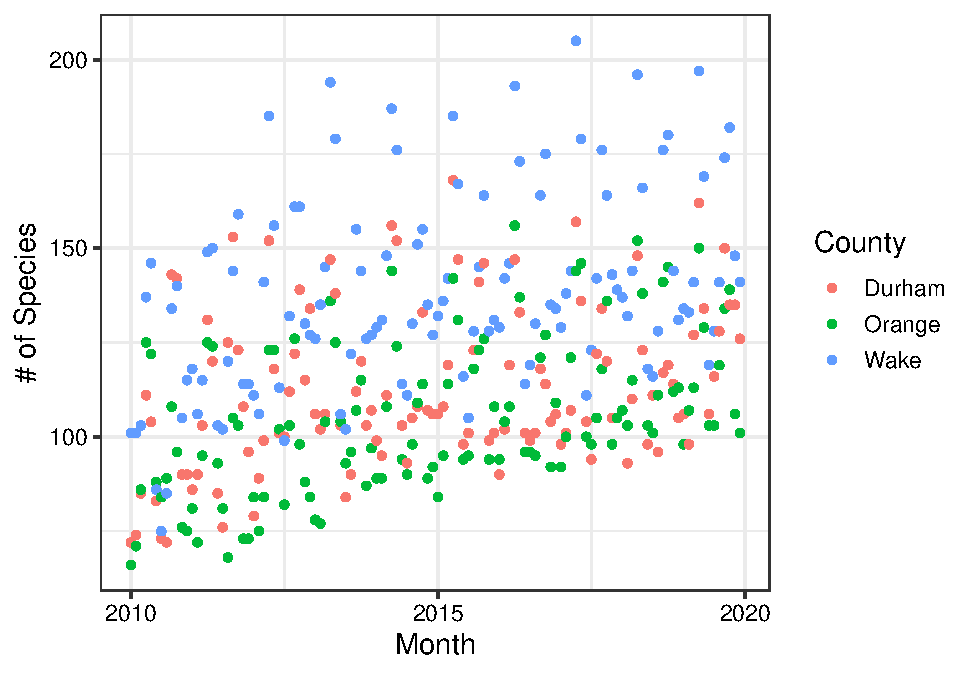
\includegraphics{Project_Template_files/figure-latex/SPP and Event Wrangling-1.pdf}
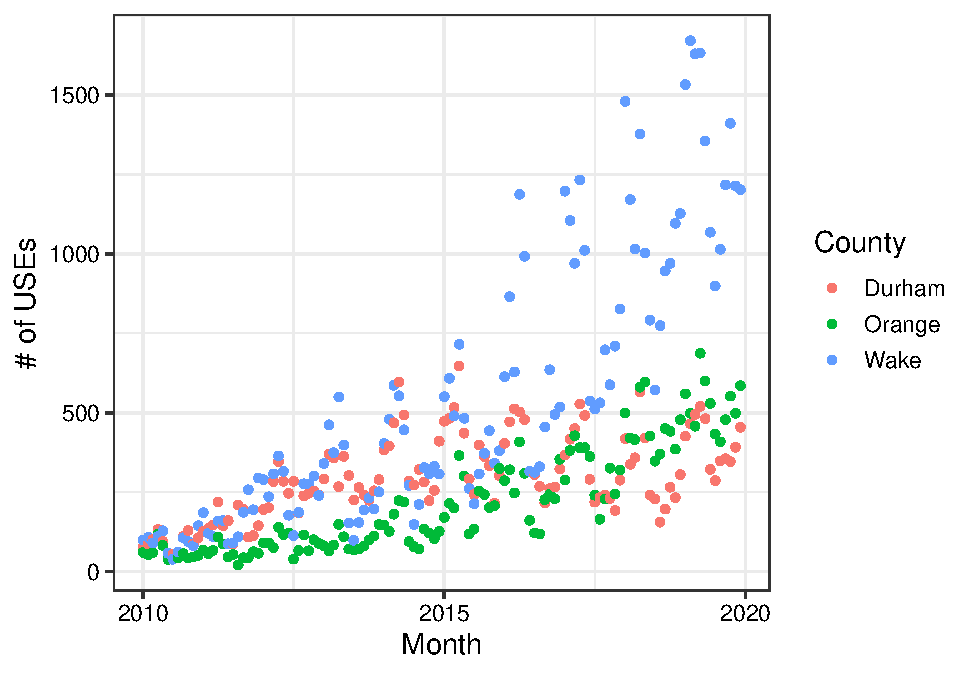
\includegraphics{Project_Template_files/figure-latex/SPP and Event Wrangling-2.pdf}

In order to perform our analysis related to species of concern in the
Research Triangle, we also used a dataset provided by the North Carolina
Wildlife Resources Commission (NCWRC) detailing Species of Greatest
Conservation Need (SGCN) in the state (NCWRC 2020). SGCN are determined
by the NCWRC based on any policies concerning threatened or endangered
species, risks related to the type of habitat they use, as well as other
indicators of concern. The raw data included information on all SGCN
identified in North Carolina, but through wrangling we filtered in order
to create a vector that only included SGCN that were birds (Table 2). By
cross-referencing this vector with the eBird data, we were able to
calculate how many SGCN were observed in each county during each year of
the decade.

\newpage

\hypertarget{exploratory-analysis}{%
\section{Exploratory Analysis}\label{exploratory-analysis}}

For our first step in analyzing our data, we created simple plots of
species richness (Figure 1) and unique sampling events (Figure 2) across
the decade to see if any clear trends could be identified. While all
three counties exhibited possible positive trends in species richness,
these were not entirely clear and required further analysis. There was a
stronger positive trend in unique sample events that was visible for all
three counties, but we also wanted to analyze this trend more precisely.

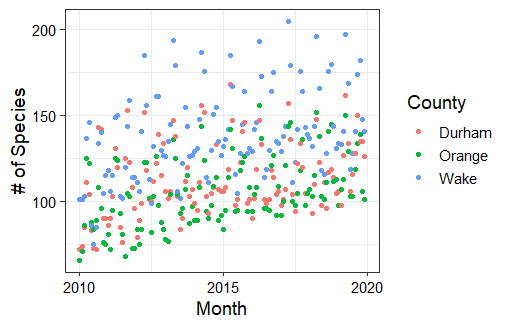
\includegraphics{./Output/EDA_SppRichness_Plot.png}
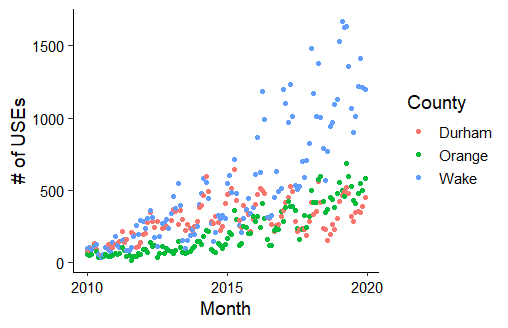
\includegraphics{./Output/EDA_EventCount_Plot.png} Since the eBird data
included latitude and longitude for every observation, the other
component of our exploratory analysis included visualizing the location
of each observation geospatially (Figure 3). This plot shows that the
distribution of sampling locations was not evenly distributed across the
region and that observations were concentrated around the urban centers
of each county (Durham, Chapel Hill, and Raleigh).

\begin{Shaded}
\begin{Highlighting}[]
\NormalTok{Durham.total }\OtherTok{\textless{}{-}} \FunctionTok{rbind}\NormalTok{(Durham}\FloatTok{.1}\NormalTok{, Durham}\FloatTok{.2}\NormalTok{)}
\NormalTok{Orange.total }\OtherTok{\textless{}{-}} \FunctionTok{rbind}\NormalTok{(Orange}\FloatTok{.1}\NormalTok{, Orange}\FloatTok{.2}\NormalTok{)}
\NormalTok{Wake.total }\OtherTok{\textless{}{-}} \FunctionTok{rbind}\NormalTok{(Wake}\FloatTok{.1}\NormalTok{, Wake}\FloatTok{.2}\NormalTok{, Wake}\FloatTok{.3}\NormalTok{)}

\NormalTok{Durham.sf }\OtherTok{\textless{}{-}}\NormalTok{ Durham.total }\SpecialCharTok{\%\textgreater{}\%}
  \FunctionTok{group\_by}\NormalTok{(LOCALITY.ID, LONGITUDE, LATITUDE) }\SpecialCharTok{\%\textgreater{}\%}
  \FunctionTok{summarize}\NormalTok{(}\AttributeTok{spp\_total =} \FunctionTok{length}\NormalTok{(}\FunctionTok{unique}\NormalTok{(COMMON.NAME))) }\SpecialCharTok{\%\textgreater{}\%}
  \FunctionTok{st\_as\_sf}\NormalTok{(}\AttributeTok{coords =} \FunctionTok{c}\NormalTok{(}\StringTok{"LONGITUDE"}\NormalTok{, }\StringTok{"LATITUDE"}\NormalTok{), }\AttributeTok{crs =} \DecValTok{4326}\NormalTok{)}
\end{Highlighting}
\end{Shaded}

\begin{verbatim}
## `summarise()` has grouped output by 'LOCALITY.ID', 'LONGITUDE'. You can override using the `.groups` argument.
\end{verbatim}

\begin{Shaded}
\begin{Highlighting}[]
\NormalTok{Orange.sf }\OtherTok{\textless{}{-}}\NormalTok{ Orange.total }\SpecialCharTok{\%\textgreater{}\%}
  \FunctionTok{group\_by}\NormalTok{(LOCALITY.ID, LONGITUDE, LATITUDE) }\SpecialCharTok{\%\textgreater{}\%}
  \FunctionTok{summarize}\NormalTok{(}\AttributeTok{spp\_total =} \FunctionTok{length}\NormalTok{(}\FunctionTok{unique}\NormalTok{(COMMON.NAME))) }\SpecialCharTok{\%\textgreater{}\%}
  \FunctionTok{st\_as\_sf}\NormalTok{(}\AttributeTok{coords =} \FunctionTok{c}\NormalTok{(}\StringTok{"LONGITUDE"}\NormalTok{, }\StringTok{"LATITUDE"}\NormalTok{), }\AttributeTok{crs =} \DecValTok{4326}\NormalTok{)}
\end{Highlighting}
\end{Shaded}

\begin{verbatim}
## `summarise()` has grouped output by 'LOCALITY.ID', 'LONGITUDE'. You can override using the `.groups` argument.
\end{verbatim}

\begin{Shaded}
\begin{Highlighting}[]
\NormalTok{Wake.sf }\OtherTok{\textless{}{-}}\NormalTok{ Wake.total }\SpecialCharTok{\%\textgreater{}\%}
  \FunctionTok{group\_by}\NormalTok{(LOCALITY.ID, LONGITUDE, LATITUDE) }\SpecialCharTok{\%\textgreater{}\%}
  \FunctionTok{summarize}\NormalTok{(}\AttributeTok{spp\_total =} \FunctionTok{length}\NormalTok{(}\FunctionTok{unique}\NormalTok{(COMMON.NAME))) }\SpecialCharTok{\%\textgreater{}\%}
  \FunctionTok{st\_as\_sf}\NormalTok{(}\AttributeTok{coords =} \FunctionTok{c}\NormalTok{(}\StringTok{"LONGITUDE"}\NormalTok{, }\StringTok{"LATITUDE"}\NormalTok{), }\AttributeTok{crs =} \DecValTok{4326}\NormalTok{)}
\end{Highlighting}
\end{Shaded}

\begin{verbatim}
## `summarise()` has grouped output by 'LOCALITY.ID', 'LONGITUDE'. You can override using the `.groups` argument.
\end{verbatim}

\begin{Shaded}
\begin{Highlighting}[]
\NormalTok{counties\_sf }\OtherTok{\textless{}{-}} \FunctionTok{st\_transform}\NormalTok{(counties\_sf, }\AttributeTok{crs =} \DecValTok{4326}\NormalTok{)}

\FunctionTok{ggplot}\NormalTok{() }\SpecialCharTok{+} \FunctionTok{geom\_sf}\NormalTok{(}\AttributeTok{data =}\NormalTok{ counties\_sf, }\FunctionTok{aes}\NormalTok{(}\AttributeTok{fill =}\NormalTok{ NAME)) }\SpecialCharTok{+} 
  \FunctionTok{geom\_sf}\NormalTok{(}\AttributeTok{data =}\NormalTok{ Durham.sf, }\AttributeTok{size =} \FloatTok{0.5}\NormalTok{) }\SpecialCharTok{+} 
  \FunctionTok{geom\_sf}\NormalTok{(}\AttributeTok{data =}\NormalTok{ Orange.sf, }\AttributeTok{size =} \FloatTok{0.5}\NormalTok{) }\SpecialCharTok{+} 
  \FunctionTok{geom\_sf}\NormalTok{(}\AttributeTok{data =}\NormalTok{ Wake.sf, }\AttributeTok{size =} \FloatTok{0.5}\NormalTok{) }\SpecialCharTok{+} \FunctionTok{labs}\NormalTok{(}\AttributeTok{fill =} \StringTok{"County"}\NormalTok{)}
\end{Highlighting}
\end{Shaded}

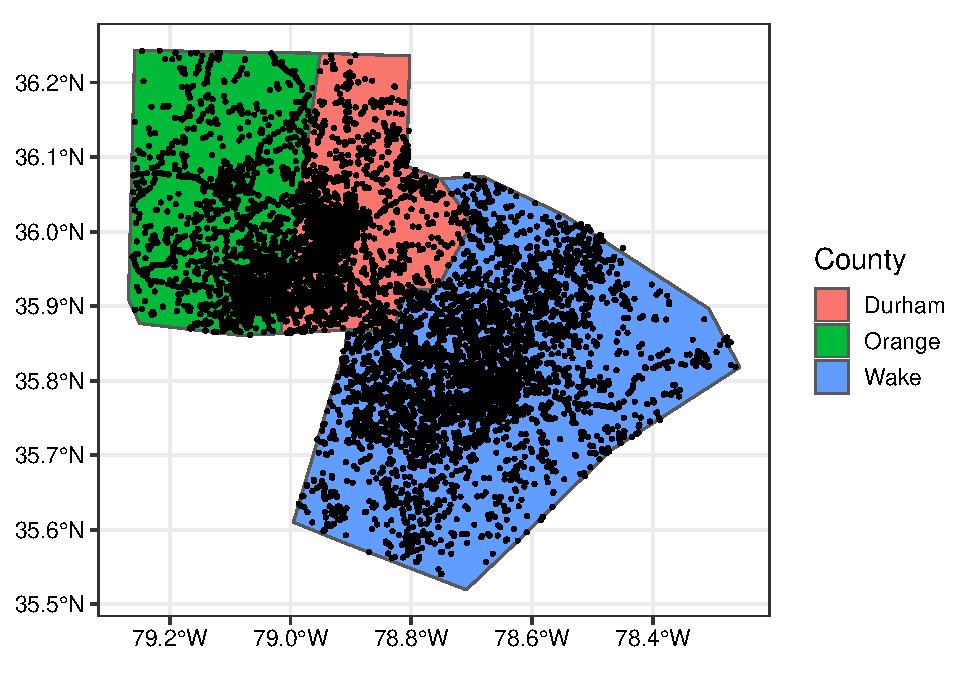
\includegraphics{Project_Template_files/figure-latex/Geospatial EDA-1.pdf}

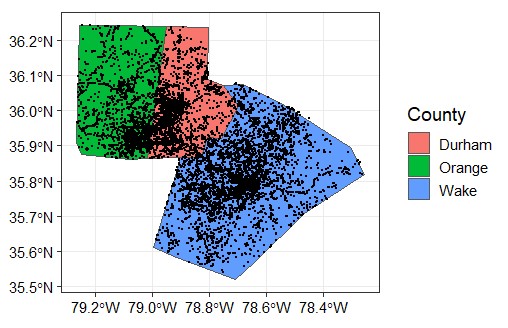
\includegraphics{./Output/EDA_geospatial_plot.png} \newpage

\hypertarget{analysis}{%
\section{Analysis}\label{analysis}}

\hypertarget{question-1-how-did-the-diversity-of-the-research-triangles-bird-population-change-during-the-2010s}{%
\subsection{Question 1: How did the diversity of the Research Triangle's
bird population change during the
2010s?}\label{question-1-how-did-the-diversity-of-the-research-triangles-bird-population-change-during-the-2010s}}

A time series analysis of species richness across all three counties
combined showed both a seasonal trend as well as a strong positive
monotonic trend (Figure 4). The seasonal trend likely correlates with
the spring and fall migration seasons when more species would be present
in the area. A seasonal Mann-Kendall test supported our identification
of a significant positive trend in species richness across the time
period (score = 195, tau = 0.366, p \textless{} 0.001).

\begin{Shaded}
\begin{Highlighting}[]
\NormalTok{total}\FloatTok{.1} \OtherTok{\textless{}{-}} \FunctionTok{rbind}\NormalTok{(Durham}\FloatTok{.1}\NormalTok{, Orange}\FloatTok{.1}\NormalTok{, Wake}\FloatTok{.1}\NormalTok{)}
\NormalTok{total}\FloatTok{.2} \OtherTok{\textless{}{-}} \FunctionTok{rbind}\NormalTok{(Durham}\FloatTok{.2}\NormalTok{, Orange}\FloatTok{.2}\NormalTok{)}
\NormalTok{total}\FloatTok{.2} \OtherTok{\textless{}{-}} \FunctionTok{rbind}\NormalTok{(total}\FloatTok{.2}\NormalTok{, Wake}\FloatTok{.2}\NormalTok{, Wake}\FloatTok{.3}\NormalTok{)}
\NormalTok{total.data }\OtherTok{\textless{}{-}} \FunctionTok{rbind}\NormalTok{(total}\FloatTok{.1}\NormalTok{, total}\FloatTok{.2}\NormalTok{)}

\NormalTok{spp.counts.total }\OtherTok{\textless{}{-}}\NormalTok{ total.data }\SpecialCharTok{\%\textgreater{}\%}
  \FunctionTok{group\_by}\NormalTok{(MY) }\SpecialCharTok{\%\textgreater{}\%}
  \FunctionTok{summarize}\NormalTok{(}\AttributeTok{spp\_total =} \FunctionTok{length}\NormalTok{(}\FunctionTok{unique}\NormalTok{(COMMON.NAME)))}

\CommentTok{\# Species richness by month}
\NormalTok{Total.ts }\OtherTok{\textless{}{-}} \FunctionTok{ts}\NormalTok{(spp.counts.total}\SpecialCharTok{$}\NormalTok{spp\_total, }\AttributeTok{start =} \FunctionTok{c}\NormalTok{(}\DecValTok{2010}\NormalTok{,}\DecValTok{1}\NormalTok{), }\AttributeTok{frequency =} \DecValTok{12}\NormalTok{)}
\NormalTok{Total.decomp }\OtherTok{\textless{}{-}} \FunctionTok{stl}\NormalTok{(Total.ts, }\AttributeTok{s.window =} \StringTok{"periodic"}\NormalTok{)}
\FunctionTok{plot}\NormalTok{(Total.decomp)}
\end{Highlighting}
\end{Shaded}

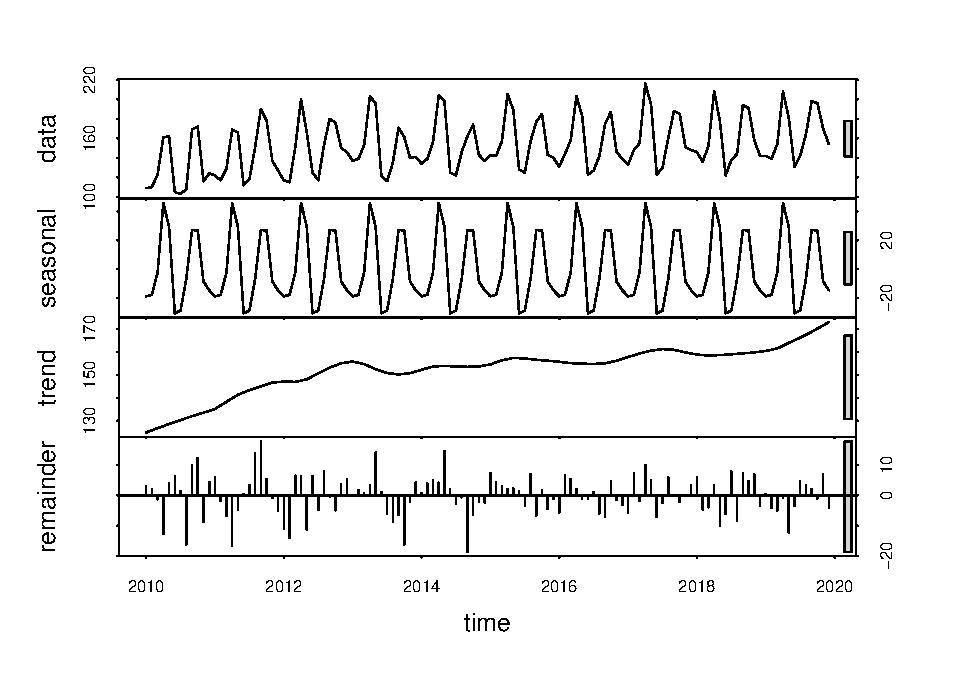
\includegraphics{Project_Template_files/figure-latex/RT SPP TS-1.pdf}

\begin{Shaded}
\begin{Highlighting}[]
\NormalTok{Total.spp.trend }\OtherTok{\textless{}{-}}\NormalTok{ Kendall}\SpecialCharTok{::}\FunctionTok{SeasonalMannKendall}\NormalTok{(Total.ts) }
\NormalTok{Total.spp.trend}
\end{Highlighting}
\end{Shaded}

\begin{verbatim}
## tau = 0.563, 2-sided pvalue =5.9952e-15
\end{verbatim}

\begin{Shaded}
\begin{Highlighting}[]
\FunctionTok{summary}\NormalTok{(Total.spp.trend)}
\end{Highlighting}
\end{Shaded}

\begin{verbatim}
## Score =  301 , Var(Score) = 1488.333
## denominator =  534.4285
## tau = 0.563, 2-sided pvalue =5.9952e-15
\end{verbatim}

\begin{figure}
\centering
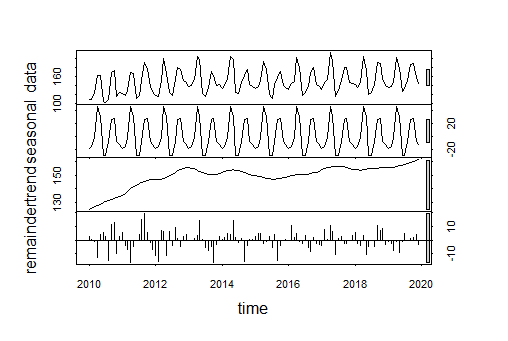
\includegraphics{./Output/RT_spp_ts_decomp.png}
\caption{Figure 4. Time series decomposition for species richness
aggregated across all three counties from 2010 to 2019.}
\end{figure}

\hypertarget{question-1a-is-this-trend-consistent-across-all-three-main-counties-in-the-region-durham-orange-and-wake}{%
\subsection{Question 1a: Is this trend consistent across all three main
counties in the region (Durham, Orange, and
Wake)?}\label{question-1a-is-this-trend-consistent-across-all-three-main-counties-in-the-region-durham-orange-and-wake}}

Individual time series analysis for each county also exhibited
seasonality as well as positive monotonic trends (Figures 5a-c). The
pattern and rate of this positive trend was slightly different among the
counties, however. While species richness saw a steeper increase earlier
in the decade in Wake County, there was a more gradual increase
throughout the period in Orange County, and Durham County saw a steeper
increase in more recent years. Seasonal Mann-Kendall tests produced
significant results for Durham (score = 172, tau = 0.322, p \textless{}
0.001), Orange (score = 381, tau = 0.710, p \textless{} 0.001), and Wake
counties (score = 345, tau = 0.650, p \textless{} 0.001).

\begin{Shaded}
\begin{Highlighting}[]
\CommentTok{\# DURHAM}
\NormalTok{Durham.ts }\OtherTok{\textless{}{-}} \FunctionTok{ts}\NormalTok{(spp.counts.Durham}\SpecialCharTok{$}\NormalTok{spp\_total, }\AttributeTok{start =} \FunctionTok{c}\NormalTok{(}\DecValTok{2010}\NormalTok{,}\DecValTok{1}\NormalTok{), }\AttributeTok{frequency =} \DecValTok{12}\NormalTok{)}
\NormalTok{Durham.decomp }\OtherTok{\textless{}{-}} \FunctionTok{stl}\NormalTok{(Durham.ts, }\AttributeTok{s.window =} \StringTok{"periodic"}\NormalTok{)}
\FunctionTok{plot}\NormalTok{(Durham.decomp)}
\end{Highlighting}
\end{Shaded}

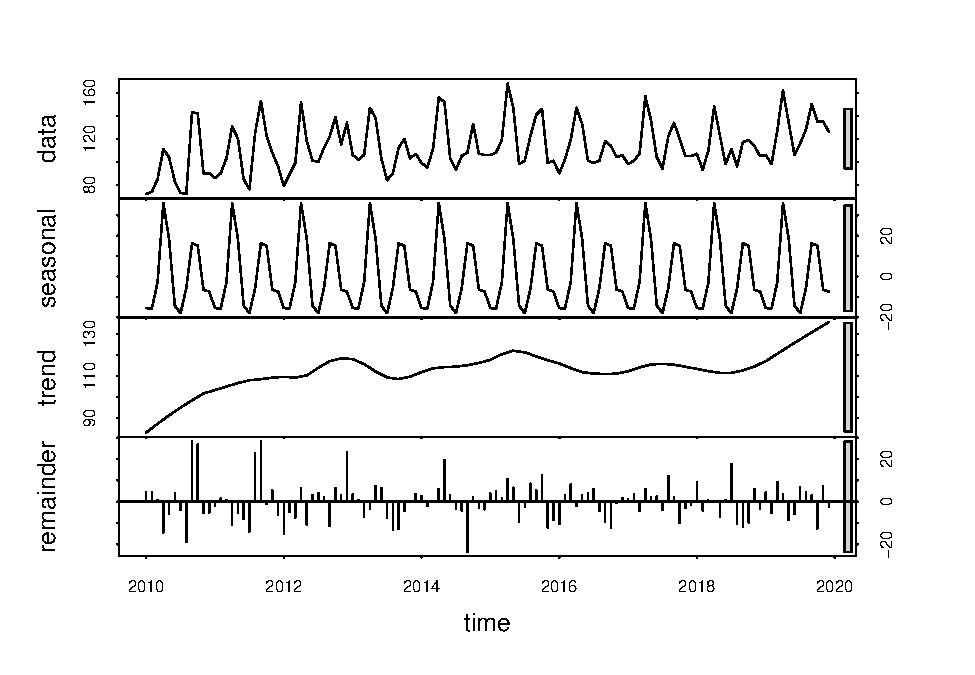
\includegraphics{Project_Template_files/figure-latex/county SPP TS-1.pdf}

\begin{Shaded}
\begin{Highlighting}[]
\NormalTok{Durham.spp.trend }\OtherTok{\textless{}{-}}\NormalTok{ Kendall}\SpecialCharTok{::}\FunctionTok{SeasonalMannKendall}\NormalTok{(Durham.ts) }
\NormalTok{Durham.spp.trend}
\end{Highlighting}
\end{Shaded}

\begin{verbatim}
## tau = 0.322, 2-sided pvalue =8.2001e-06
\end{verbatim}

\begin{Shaded}
\begin{Highlighting}[]
\FunctionTok{summary}\NormalTok{(Durham.spp.trend)}
\end{Highlighting}
\end{Shaded}

\begin{verbatim}
## Score =  172 , Var(Score) = 1487.333
## denominator =  533.9257
## tau = 0.322, 2-sided pvalue =8.2001e-06
\end{verbatim}

\begin{Shaded}
\begin{Highlighting}[]
\CommentTok{\# ORANGE}
\NormalTok{Orange.ts }\OtherTok{\textless{}{-}} \FunctionTok{ts}\NormalTok{(spp.counts.Orange}\SpecialCharTok{$}\NormalTok{spp\_total, }\AttributeTok{start =} \FunctionTok{c}\NormalTok{(}\DecValTok{2010}\NormalTok{,}\DecValTok{1}\NormalTok{), }\AttributeTok{frequency =} \DecValTok{12}\NormalTok{)}
\NormalTok{Orange.decomp }\OtherTok{\textless{}{-}} \FunctionTok{stl}\NormalTok{(Orange.ts, }\AttributeTok{s.window =} \StringTok{"periodic"}\NormalTok{)}
\FunctionTok{plot}\NormalTok{(Orange.decomp)}
\end{Highlighting}
\end{Shaded}

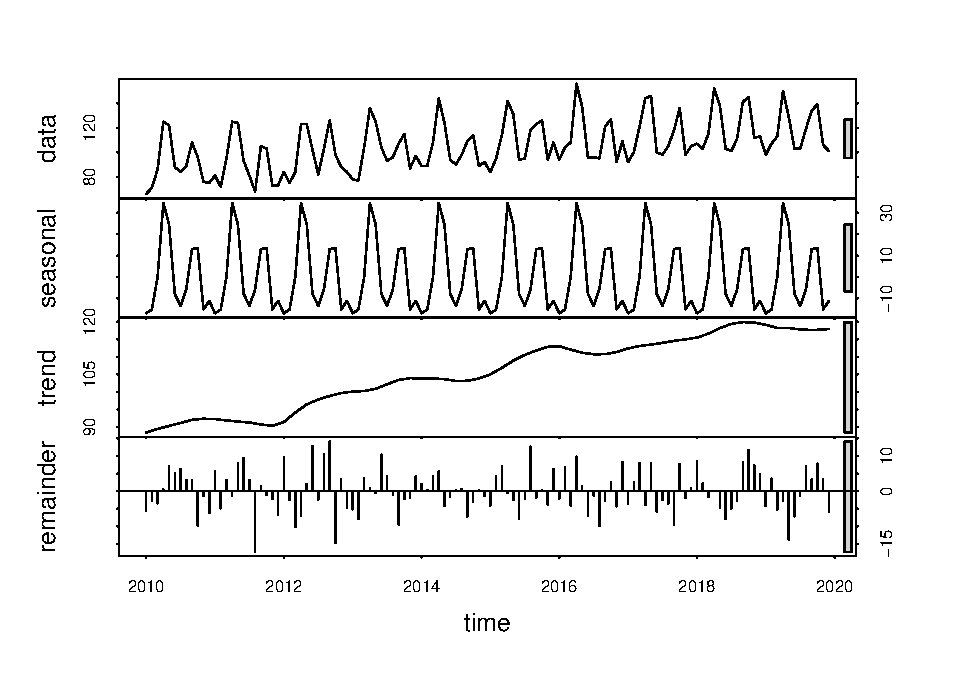
\includegraphics{Project_Template_files/figure-latex/county SPP TS-2.pdf}

\begin{Shaded}
\begin{Highlighting}[]
\NormalTok{Orange.spp.trend }\OtherTok{\textless{}{-}}\NormalTok{ Kendall}\SpecialCharTok{::}\FunctionTok{SeasonalMannKendall}\NormalTok{(Orange.ts) }
\NormalTok{Orange.spp.trend}
\end{Highlighting}
\end{Shaded}

\begin{verbatim}
## tau = 0.71, 2-sided pvalue =< 2.22e-16
\end{verbatim}

\begin{Shaded}
\begin{Highlighting}[]
\FunctionTok{summary}\NormalTok{(Orange.spp.trend)}
\end{Highlighting}
\end{Shaded}

\begin{verbatim}
## Score =  381 , Var(Score) = 1493
## denominator =  536.4688
## tau = 0.71, 2-sided pvalue =< 2.22e-16
\end{verbatim}

\begin{Shaded}
\begin{Highlighting}[]
\CommentTok{\# WAKE}
\NormalTok{Wake.ts }\OtherTok{\textless{}{-}} \FunctionTok{ts}\NormalTok{(spp.counts.Wake}\SpecialCharTok{$}\NormalTok{spp\_total, }\AttributeTok{start =} \FunctionTok{c}\NormalTok{(}\DecValTok{2010}\NormalTok{,}\DecValTok{1}\NormalTok{), }\AttributeTok{frequency =} \DecValTok{12}\NormalTok{)}
\NormalTok{Wake.decomp }\OtherTok{\textless{}{-}} \FunctionTok{stl}\NormalTok{(Wake.ts, }\AttributeTok{s.window =} \StringTok{"periodic"}\NormalTok{)}
\FunctionTok{plot}\NormalTok{(Wake.decomp)}
\end{Highlighting}
\end{Shaded}

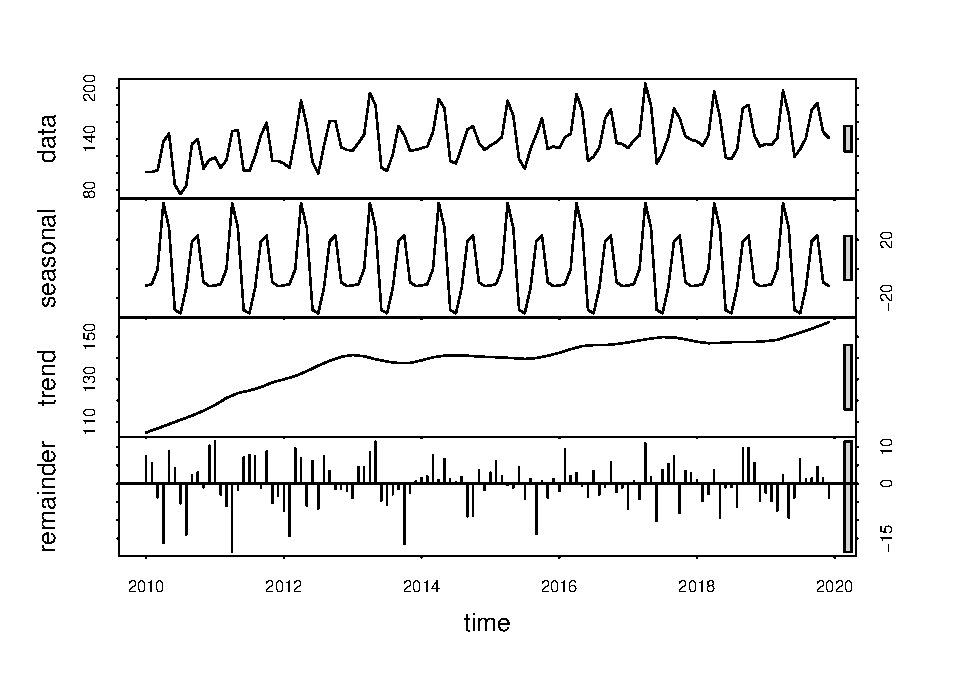
\includegraphics{Project_Template_files/figure-latex/county SPP TS-3.pdf}

\begin{Shaded}
\begin{Highlighting}[]
\NormalTok{Wake.spp.trend }\OtherTok{\textless{}{-}}\NormalTok{ Kendall}\SpecialCharTok{::}\FunctionTok{SeasonalMannKendall}\NormalTok{(Wake.ts) }
\NormalTok{Wake.spp.trend}
\end{Highlighting}
\end{Shaded}

\begin{verbatim}
## tau = 0.65, 2-sided pvalue =< 2.22e-16
\end{verbatim}

\begin{Shaded}
\begin{Highlighting}[]
\FunctionTok{summary}\NormalTok{(Wake.spp.trend)}
\end{Highlighting}
\end{Shaded}

\begin{verbatim}
## Score =  345 , Var(Score) = 1479.667
## denominator =  530.3824
## tau = 0.65, 2-sided pvalue =< 2.22e-16
\end{verbatim}

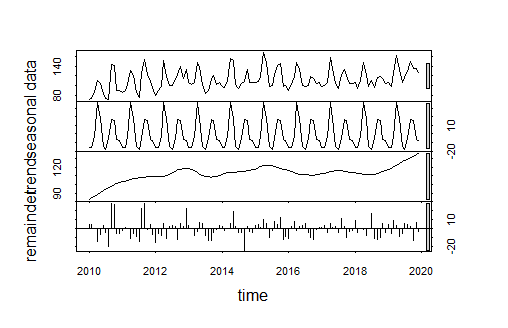
\includegraphics{./Output/Durham_spp_ts_decomp.png}
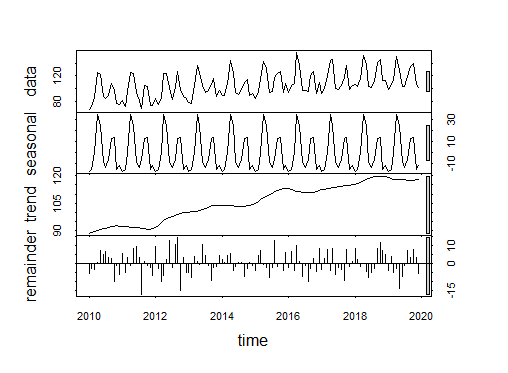
\includegraphics{./Output/Orange_spp_ts_decomp.png}
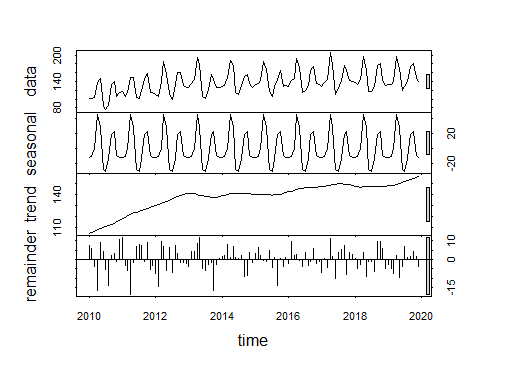
\includegraphics{./Output/Wake_spp_ts_decomp.png}

\hypertarget{question-1b-was-there-a-clear-trend-in-the-presence-of-species-of-concern-across-the-decade}{%
\subsection{Question 1b: Was there a clear trend in the presence of
species of concern across the
decade?}\label{question-1b-was-there-a-clear-trend-in-the-presence-of-species-of-concern-across-the-decade}}

For each of the three counties, the number of SGCN observed in the final
year of the period (2019) was noticeably higher than the number observed
in the first year of the period (2010; Figure 6). However, none of the
counties exhibited a constant increase in SGCN count across the entire
decade, suggesting that further analysis is necessary to fully
understand the trend in these data.

\begin{Shaded}
\begin{Highlighting}[]
\NormalTok{Durham.total }\OtherTok{\textless{}{-}}\NormalTok{ Durham.total }\SpecialCharTok{\%\textgreater{}\%}
  \FunctionTok{mutate}\NormalTok{(}\AttributeTok{SGCN =} \FunctionTok{ifelse}\NormalTok{(COMMON.NAME }\SpecialCharTok{\%in\%}\NormalTok{ SGCN\_bird\_list, }\StringTok{"Y"}\NormalTok{, }\StringTok{"N"}\NormalTok{))}

\NormalTok{Durham.SGCN }\OtherTok{\textless{}{-}} \FunctionTok{unique}\NormalTok{(Durham.total}\SpecialCharTok{$}\NormalTok{COMMON.NAME[Durham.total}\SpecialCharTok{$}\NormalTok{SGCN }\SpecialCharTok{==} \StringTok{"Y"}\NormalTok{])}

\FunctionTok{length}\NormalTok{(}\FunctionTok{unique}\NormalTok{(Durham.total}\SpecialCharTok{$}\NormalTok{COMMON.NAME[Durham.total}\SpecialCharTok{$}\NormalTok{SGCN }\SpecialCharTok{==} \StringTok{"Y"} \SpecialCharTok{\&}\NormalTok{ Durham.total}\SpecialCharTok{$}\NormalTok{YEAR }\SpecialCharTok{==} \DecValTok{2010}\NormalTok{]))}
\end{Highlighting}
\end{Shaded}

\begin{verbatim}
## [1] 34
\end{verbatim}

\begin{Shaded}
\begin{Highlighting}[]
\FunctionTok{length}\NormalTok{(}\FunctionTok{unique}\NormalTok{(Durham.total}\SpecialCharTok{$}\NormalTok{COMMON.NAME[Durham.total}\SpecialCharTok{$}\NormalTok{SGCN }\SpecialCharTok{==} \StringTok{"Y"} \SpecialCharTok{\&}\NormalTok{ Durham.total}\SpecialCharTok{$}\NormalTok{YEAR }\SpecialCharTok{==} \DecValTok{2011}\NormalTok{]))}
\end{Highlighting}
\end{Shaded}

\begin{verbatim}
## [1] 50
\end{verbatim}

\begin{Shaded}
\begin{Highlighting}[]
\FunctionTok{length}\NormalTok{(}\FunctionTok{unique}\NormalTok{(Durham.total}\SpecialCharTok{$}\NormalTok{COMMON.NAME[Durham.total}\SpecialCharTok{$}\NormalTok{SGCN }\SpecialCharTok{==} \StringTok{"Y"} \SpecialCharTok{\&}\NormalTok{ Durham.total}\SpecialCharTok{$}\NormalTok{YEAR }\SpecialCharTok{==} \DecValTok{2012}\NormalTok{]))}
\end{Highlighting}
\end{Shaded}

\begin{verbatim}
## [1] 40
\end{verbatim}

\begin{Shaded}
\begin{Highlighting}[]
\FunctionTok{length}\NormalTok{(}\FunctionTok{unique}\NormalTok{(Durham.total}\SpecialCharTok{$}\NormalTok{COMMON.NAME[Durham.total}\SpecialCharTok{$}\NormalTok{SGCN }\SpecialCharTok{==} \StringTok{"Y"} \SpecialCharTok{\&}\NormalTok{ Durham.total}\SpecialCharTok{$}\NormalTok{YEAR }\SpecialCharTok{==} \DecValTok{2013}\NormalTok{]))}
\end{Highlighting}
\end{Shaded}

\begin{verbatim}
## [1] 35
\end{verbatim}

\begin{Shaded}
\begin{Highlighting}[]
\FunctionTok{length}\NormalTok{(}\FunctionTok{unique}\NormalTok{(Durham.total}\SpecialCharTok{$}\NormalTok{COMMON.NAME[Durham.total}\SpecialCharTok{$}\NormalTok{SGCN }\SpecialCharTok{==} \StringTok{"Y"} \SpecialCharTok{\&}\NormalTok{ Durham.total}\SpecialCharTok{$}\NormalTok{YEAR }\SpecialCharTok{==} \DecValTok{2014}\NormalTok{]))}
\end{Highlighting}
\end{Shaded}

\begin{verbatim}
## [1] 36
\end{verbatim}

\begin{Shaded}
\begin{Highlighting}[]
\FunctionTok{length}\NormalTok{(}\FunctionTok{unique}\NormalTok{(Durham.total}\SpecialCharTok{$}\NormalTok{COMMON.NAME[Durham.total}\SpecialCharTok{$}\NormalTok{SGCN }\SpecialCharTok{==} \StringTok{"Y"} \SpecialCharTok{\&}\NormalTok{ Durham.total}\SpecialCharTok{$}\NormalTok{YEAR }\SpecialCharTok{==} \DecValTok{2015}\NormalTok{]))}
\end{Highlighting}
\end{Shaded}

\begin{verbatim}
## [1] 43
\end{verbatim}

\begin{Shaded}
\begin{Highlighting}[]
\FunctionTok{length}\NormalTok{(}\FunctionTok{unique}\NormalTok{(Durham.total}\SpecialCharTok{$}\NormalTok{COMMON.NAME[Durham.total}\SpecialCharTok{$}\NormalTok{SGCN }\SpecialCharTok{==} \StringTok{"Y"} \SpecialCharTok{\&}\NormalTok{ Durham.total}\SpecialCharTok{$}\NormalTok{YEAR }\SpecialCharTok{==} \DecValTok{2016}\NormalTok{]))}
\end{Highlighting}
\end{Shaded}

\begin{verbatim}
## [1] 35
\end{verbatim}

\begin{Shaded}
\begin{Highlighting}[]
\FunctionTok{length}\NormalTok{(}\FunctionTok{unique}\NormalTok{(Durham.total}\SpecialCharTok{$}\NormalTok{COMMON.NAME[Durham.total}\SpecialCharTok{$}\NormalTok{SGCN }\SpecialCharTok{==} \StringTok{"Y"} \SpecialCharTok{\&}\NormalTok{ Durham.total}\SpecialCharTok{$}\NormalTok{YEAR }\SpecialCharTok{==} \DecValTok{2017}\NormalTok{]))}
\end{Highlighting}
\end{Shaded}

\begin{verbatim}
## [1] 40
\end{verbatim}

\begin{Shaded}
\begin{Highlighting}[]
\FunctionTok{length}\NormalTok{(}\FunctionTok{unique}\NormalTok{(Durham.total}\SpecialCharTok{$}\NormalTok{COMMON.NAME[Durham.total}\SpecialCharTok{$}\NormalTok{SGCN }\SpecialCharTok{==} \StringTok{"Y"} \SpecialCharTok{\&}\NormalTok{ Durham.total}\SpecialCharTok{$}\NormalTok{YEAR }\SpecialCharTok{==} \DecValTok{2018}\NormalTok{]))}
\end{Highlighting}
\end{Shaded}

\begin{verbatim}
## [1] 43
\end{verbatim}

\begin{Shaded}
\begin{Highlighting}[]
\FunctionTok{length}\NormalTok{(}\FunctionTok{unique}\NormalTok{(Durham.total}\SpecialCharTok{$}\NormalTok{COMMON.NAME[Durham.total}\SpecialCharTok{$}\NormalTok{SGCN }\SpecialCharTok{==} \StringTok{"Y"} \SpecialCharTok{\&}\NormalTok{ Durham.total}\SpecialCharTok{$}\NormalTok{YEAR }\SpecialCharTok{==} \DecValTok{2019}\NormalTok{]))}
\end{Highlighting}
\end{Shaded}

\begin{verbatim}
## [1] 47
\end{verbatim}

\begin{Shaded}
\begin{Highlighting}[]
\NormalTok{Du.SGCN.counts }\OtherTok{\textless{}{-}} \FunctionTok{c}\NormalTok{(}\DecValTok{34}\NormalTok{, }\DecValTok{50}\NormalTok{, }\DecValTok{40}\NormalTok{, }\DecValTok{35}\NormalTok{, }\DecValTok{36}\NormalTok{, }\DecValTok{43}\NormalTok{, }\DecValTok{35}\NormalTok{, }\DecValTok{40}\NormalTok{, }\DecValTok{43}\NormalTok{, }\DecValTok{47}\NormalTok{)}
\NormalTok{Du.SGCN.years }\OtherTok{\textless{}{-}} \FunctionTok{c}\NormalTok{(}\DecValTok{2010}\SpecialCharTok{:}\DecValTok{2019}\NormalTok{)}
\NormalTok{Du.SGCN.by.year }\OtherTok{\textless{}{-}} \FunctionTok{cbind}\NormalTok{(Du.SGCN.years, Du.SGCN.counts)}
\FunctionTok{colnames}\NormalTok{(Du.SGCN.by.year) }\OtherTok{\textless{}{-}} \FunctionTok{c}\NormalTok{(}\StringTok{"Year"}\NormalTok{, }\StringTok{"SGCN\_total"}\NormalTok{)}
  \CommentTok{\# write.csv(Du.SGCN.by.year, "./Data/Processed/Durham\_SGCNcounts.csv")}

\NormalTok{Du.SGCN }\OtherTok{\textless{}{-}} \FunctionTok{read.csv}\NormalTok{(}\StringTok{"./Data/Processed/Durham\_SGCNcounts.csv"}\NormalTok{)}

\NormalTok{Orange.total }\OtherTok{\textless{}{-}}\NormalTok{ Orange.total }\SpecialCharTok{\%\textgreater{}\%}
  \FunctionTok{mutate}\NormalTok{(}\AttributeTok{SGCN =} \FunctionTok{ifelse}\NormalTok{(COMMON.NAME }\SpecialCharTok{\%in\%}\NormalTok{ SGCN\_bird\_list, }\StringTok{"Y"}\NormalTok{, }\StringTok{"N"}\NormalTok{))}

\NormalTok{Orange.SGCN }\OtherTok{\textless{}{-}} \FunctionTok{unique}\NormalTok{(Orange.total}\SpecialCharTok{$}\NormalTok{COMMON.NAME[Orange.total}\SpecialCharTok{$}\NormalTok{SGCN }\SpecialCharTok{==} \StringTok{"Y"}\NormalTok{])}

\CommentTok{\# The not as elegant way since pipe isn\textquotesingle{}t working...}

\FunctionTok{length}\NormalTok{(}\FunctionTok{unique}\NormalTok{(Orange.total}\SpecialCharTok{$}\NormalTok{COMMON.NAME[Orange.total}\SpecialCharTok{$}\NormalTok{SGCN }\SpecialCharTok{==} \StringTok{"Y"} \SpecialCharTok{\&}\NormalTok{ Orange.total}\SpecialCharTok{$}\NormalTok{YEAR }\SpecialCharTok{==} \DecValTok{2010}\NormalTok{]))}
\end{Highlighting}
\end{Shaded}

\begin{verbatim}
## [1] 26
\end{verbatim}

\begin{Shaded}
\begin{Highlighting}[]
\FunctionTok{length}\NormalTok{(}\FunctionTok{unique}\NormalTok{(Orange.total}\SpecialCharTok{$}\NormalTok{COMMON.NAME[Orange.total}\SpecialCharTok{$}\NormalTok{SGCN }\SpecialCharTok{==} \StringTok{"Y"} \SpecialCharTok{\&}\NormalTok{ Orange.total}\SpecialCharTok{$}\NormalTok{YEAR }\SpecialCharTok{==} \DecValTok{2011}\NormalTok{]))}
\end{Highlighting}
\end{Shaded}

\begin{verbatim}
## [1] 23
\end{verbatim}

\begin{Shaded}
\begin{Highlighting}[]
\FunctionTok{length}\NormalTok{(}\FunctionTok{unique}\NormalTok{(Orange.total}\SpecialCharTok{$}\NormalTok{COMMON.NAME[Orange.total}\SpecialCharTok{$}\NormalTok{SGCN }\SpecialCharTok{==} \StringTok{"Y"} \SpecialCharTok{\&}\NormalTok{ Orange.total}\SpecialCharTok{$}\NormalTok{YEAR }\SpecialCharTok{==} \DecValTok{2012}\NormalTok{]))}
\end{Highlighting}
\end{Shaded}

\begin{verbatim}
## [1] 25
\end{verbatim}

\begin{Shaded}
\begin{Highlighting}[]
\FunctionTok{length}\NormalTok{(}\FunctionTok{unique}\NormalTok{(Orange.total}\SpecialCharTok{$}\NormalTok{COMMON.NAME[Orange.total}\SpecialCharTok{$}\NormalTok{SGCN }\SpecialCharTok{==} \StringTok{"Y"} \SpecialCharTok{\&}\NormalTok{ Orange.total}\SpecialCharTok{$}\NormalTok{YEAR }\SpecialCharTok{==} \DecValTok{2013}\NormalTok{]))}
\end{Highlighting}
\end{Shaded}

\begin{verbatim}
## [1] 29
\end{verbatim}

\begin{Shaded}
\begin{Highlighting}[]
\FunctionTok{length}\NormalTok{(}\FunctionTok{unique}\NormalTok{(Orange.total}\SpecialCharTok{$}\NormalTok{COMMON.NAME[Orange.total}\SpecialCharTok{$}\NormalTok{SGCN }\SpecialCharTok{==} \StringTok{"Y"} \SpecialCharTok{\&}\NormalTok{ Orange.total}\SpecialCharTok{$}\NormalTok{YEAR }\SpecialCharTok{==} \DecValTok{2014}\NormalTok{]))}
\end{Highlighting}
\end{Shaded}

\begin{verbatim}
## [1] 31
\end{verbatim}

\begin{Shaded}
\begin{Highlighting}[]
\FunctionTok{length}\NormalTok{(}\FunctionTok{unique}\NormalTok{(Orange.total}\SpecialCharTok{$}\NormalTok{COMMON.NAME[Orange.total}\SpecialCharTok{$}\NormalTok{SGCN }\SpecialCharTok{==} \StringTok{"Y"} \SpecialCharTok{\&}\NormalTok{ Orange.total}\SpecialCharTok{$}\NormalTok{YEAR }\SpecialCharTok{==} \DecValTok{2015}\NormalTok{]))}
\end{Highlighting}
\end{Shaded}

\begin{verbatim}
## [1] 33
\end{verbatim}

\begin{Shaded}
\begin{Highlighting}[]
\FunctionTok{length}\NormalTok{(}\FunctionTok{unique}\NormalTok{(Orange.total}\SpecialCharTok{$}\NormalTok{COMMON.NAME[Orange.total}\SpecialCharTok{$}\NormalTok{SGCN }\SpecialCharTok{==} \StringTok{"Y"} \SpecialCharTok{\&}\NormalTok{ Orange.total}\SpecialCharTok{$}\NormalTok{YEAR }\SpecialCharTok{==} \DecValTok{2016}\NormalTok{]))}
\end{Highlighting}
\end{Shaded}

\begin{verbatim}
## [1] 32
\end{verbatim}

\begin{Shaded}
\begin{Highlighting}[]
\FunctionTok{length}\NormalTok{(}\FunctionTok{unique}\NormalTok{(Orange.total}\SpecialCharTok{$}\NormalTok{COMMON.NAME[Orange.total}\SpecialCharTok{$}\NormalTok{SGCN }\SpecialCharTok{==} \StringTok{"Y"} \SpecialCharTok{\&}\NormalTok{ Orange.total}\SpecialCharTok{$}\NormalTok{YEAR }\SpecialCharTok{==} \DecValTok{2017}\NormalTok{]))}
\end{Highlighting}
\end{Shaded}

\begin{verbatim}
## [1] 32
\end{verbatim}

\begin{Shaded}
\begin{Highlighting}[]
\FunctionTok{length}\NormalTok{(}\FunctionTok{unique}\NormalTok{(Orange.total}\SpecialCharTok{$}\NormalTok{COMMON.NAME[Orange.total}\SpecialCharTok{$}\NormalTok{SGCN }\SpecialCharTok{==} \StringTok{"Y"} \SpecialCharTok{\&}\NormalTok{ Orange.total}\SpecialCharTok{$}\NormalTok{YEAR }\SpecialCharTok{==} \DecValTok{2018}\NormalTok{]))}
\end{Highlighting}
\end{Shaded}

\begin{verbatim}
## [1] 33
\end{verbatim}

\begin{Shaded}
\begin{Highlighting}[]
\FunctionTok{length}\NormalTok{(}\FunctionTok{unique}\NormalTok{(Orange.total}\SpecialCharTok{$}\NormalTok{COMMON.NAME[Orange.total}\SpecialCharTok{$}\NormalTok{SGCN }\SpecialCharTok{==} \StringTok{"Y"} \SpecialCharTok{\&}\NormalTok{ Orange.total}\SpecialCharTok{$}\NormalTok{YEAR }\SpecialCharTok{==} \DecValTok{2019}\NormalTok{]))}
\end{Highlighting}
\end{Shaded}

\begin{verbatim}
## [1] 31
\end{verbatim}

\begin{Shaded}
\begin{Highlighting}[]
\NormalTok{Or.SGCN.counts }\OtherTok{\textless{}{-}} \FunctionTok{c}\NormalTok{(}\DecValTok{26}\NormalTok{, }\DecValTok{23}\NormalTok{, }\DecValTok{25}\NormalTok{, }\DecValTok{29}\NormalTok{, }\DecValTok{31}\NormalTok{, }\DecValTok{33}\NormalTok{, }\DecValTok{32}\NormalTok{, }\DecValTok{32}\NormalTok{, }\DecValTok{33}\NormalTok{, }\DecValTok{31}\NormalTok{)}
\NormalTok{Or.SGCN.years }\OtherTok{\textless{}{-}} \FunctionTok{c}\NormalTok{(}\DecValTok{2010}\SpecialCharTok{:}\DecValTok{2019}\NormalTok{)}
\NormalTok{Or.SGCN.by.year }\OtherTok{\textless{}{-}} \FunctionTok{cbind}\NormalTok{(Or.SGCN.years, Or.SGCN.counts)}
\FunctionTok{colnames}\NormalTok{(Or.SGCN.by.year) }\OtherTok{\textless{}{-}} \FunctionTok{c}\NormalTok{(}\StringTok{"Year"}\NormalTok{, }\StringTok{"SGCN\_total"}\NormalTok{)}
  \CommentTok{\# write.csv(Or.SGCN.by.year, "./Data/Processed/Orange\_SGCNcounts.csv")}

\NormalTok{Or.SGCN }\OtherTok{\textless{}{-}} \FunctionTok{read.csv}\NormalTok{(}\StringTok{"./Data/Processed/Orange\_SGCNcounts.csv"}\NormalTok{)}

\NormalTok{Wake.total }\OtherTok{\textless{}{-}}\NormalTok{ Wake.total }\SpecialCharTok{\%\textgreater{}\%}
  \FunctionTok{mutate}\NormalTok{(}\AttributeTok{SGCN =} \FunctionTok{ifelse}\NormalTok{(COMMON.NAME }\SpecialCharTok{\%in\%}\NormalTok{ SGCN\_bird\_list, }\StringTok{"Y"}\NormalTok{, }\StringTok{"N"}\NormalTok{))}

\NormalTok{Wake.SGCN }\OtherTok{\textless{}{-}} \FunctionTok{unique}\NormalTok{(Wake.total}\SpecialCharTok{$}\NormalTok{COMMON.NAME[Wake.total}\SpecialCharTok{$}\NormalTok{SGCN }\SpecialCharTok{==} \StringTok{"Y"}\NormalTok{])}

\CommentTok{\# The not as elegant way since pipe isn\textquotesingle{}t working...}

\FunctionTok{length}\NormalTok{(}\FunctionTok{unique}\NormalTok{(Wake.total}\SpecialCharTok{$}\NormalTok{COMMON.NAME[Wake.total}\SpecialCharTok{$}\NormalTok{SGCN }\SpecialCharTok{==} \StringTok{"Y"} \SpecialCharTok{\&}\NormalTok{ Wake.total}\SpecialCharTok{$}\NormalTok{YEAR }\SpecialCharTok{==} \DecValTok{2010}\NormalTok{]))}
\end{Highlighting}
\end{Shaded}

\begin{verbatim}
## [1] 38
\end{verbatim}

\begin{Shaded}
\begin{Highlighting}[]
\FunctionTok{length}\NormalTok{(}\FunctionTok{unique}\NormalTok{(Wake.total}\SpecialCharTok{$}\NormalTok{COMMON.NAME[Wake.total}\SpecialCharTok{$}\NormalTok{SGCN }\SpecialCharTok{==} \StringTok{"Y"} \SpecialCharTok{\&}\NormalTok{ Wake.total}\SpecialCharTok{$}\NormalTok{YEAR }\SpecialCharTok{==} \DecValTok{2011}\NormalTok{]))}
\end{Highlighting}
\end{Shaded}

\begin{verbatim}
## [1] 42
\end{verbatim}

\begin{Shaded}
\begin{Highlighting}[]
\FunctionTok{length}\NormalTok{(}\FunctionTok{unique}\NormalTok{(Wake.total}\SpecialCharTok{$}\NormalTok{COMMON.NAME[Wake.total}\SpecialCharTok{$}\NormalTok{SGCN }\SpecialCharTok{==} \StringTok{"Y"} \SpecialCharTok{\&}\NormalTok{ Wake.total}\SpecialCharTok{$}\NormalTok{YEAR }\SpecialCharTok{==} \DecValTok{2012}\NormalTok{]))}
\end{Highlighting}
\end{Shaded}

\begin{verbatim}
## [1] 46
\end{verbatim}

\begin{Shaded}
\begin{Highlighting}[]
\FunctionTok{length}\NormalTok{(}\FunctionTok{unique}\NormalTok{(Wake.total}\SpecialCharTok{$}\NormalTok{COMMON.NAME[Wake.total}\SpecialCharTok{$}\NormalTok{SGCN }\SpecialCharTok{==} \StringTok{"Y"} \SpecialCharTok{\&}\NormalTok{ Wake.total}\SpecialCharTok{$}\NormalTok{YEAR }\SpecialCharTok{==} \DecValTok{2013}\NormalTok{]))}
\end{Highlighting}
\end{Shaded}

\begin{verbatim}
## [1] 49
\end{verbatim}

\begin{Shaded}
\begin{Highlighting}[]
\FunctionTok{length}\NormalTok{(}\FunctionTok{unique}\NormalTok{(Wake.total}\SpecialCharTok{$}\NormalTok{COMMON.NAME[Wake.total}\SpecialCharTok{$}\NormalTok{SGCN }\SpecialCharTok{==} \StringTok{"Y"} \SpecialCharTok{\&}\NormalTok{ Wake.total}\SpecialCharTok{$}\NormalTok{YEAR }\SpecialCharTok{==} \DecValTok{2014}\NormalTok{]))}
\end{Highlighting}
\end{Shaded}

\begin{verbatim}
## [1] 43
\end{verbatim}

\begin{Shaded}
\begin{Highlighting}[]
\FunctionTok{length}\NormalTok{(}\FunctionTok{unique}\NormalTok{(Wake.total}\SpecialCharTok{$}\NormalTok{COMMON.NAME[Wake.total}\SpecialCharTok{$}\NormalTok{SGCN }\SpecialCharTok{==} \StringTok{"Y"} \SpecialCharTok{\&}\NormalTok{ Wake.total}\SpecialCharTok{$}\NormalTok{YEAR }\SpecialCharTok{==} \DecValTok{2015}\NormalTok{]))}
\end{Highlighting}
\end{Shaded}

\begin{verbatim}
## [1] 48
\end{verbatim}

\begin{Shaded}
\begin{Highlighting}[]
\FunctionTok{length}\NormalTok{(}\FunctionTok{unique}\NormalTok{(Wake.total}\SpecialCharTok{$}\NormalTok{COMMON.NAME[Wake.total}\SpecialCharTok{$}\NormalTok{SGCN }\SpecialCharTok{==} \StringTok{"Y"} \SpecialCharTok{\&}\NormalTok{ Wake.total}\SpecialCharTok{$}\NormalTok{YEAR }\SpecialCharTok{==} \DecValTok{2016}\NormalTok{]))}
\end{Highlighting}
\end{Shaded}

\begin{verbatim}
## [1] 49
\end{verbatim}

\begin{Shaded}
\begin{Highlighting}[]
\FunctionTok{length}\NormalTok{(}\FunctionTok{unique}\NormalTok{(Wake.total}\SpecialCharTok{$}\NormalTok{COMMON.NAME[Wake.total}\SpecialCharTok{$}\NormalTok{SGCN }\SpecialCharTok{==} \StringTok{"Y"} \SpecialCharTok{\&}\NormalTok{ Wake.total}\SpecialCharTok{$}\NormalTok{YEAR }\SpecialCharTok{==} \DecValTok{2017}\NormalTok{]))}
\end{Highlighting}
\end{Shaded}

\begin{verbatim}
## [1] 45
\end{verbatim}

\begin{Shaded}
\begin{Highlighting}[]
\FunctionTok{length}\NormalTok{(}\FunctionTok{unique}\NormalTok{(Wake.total}\SpecialCharTok{$}\NormalTok{COMMON.NAME[Wake.total}\SpecialCharTok{$}\NormalTok{SGCN }\SpecialCharTok{==} \StringTok{"Y"} \SpecialCharTok{\&}\NormalTok{ Wake.total}\SpecialCharTok{$}\NormalTok{YEAR }\SpecialCharTok{==} \DecValTok{2018}\NormalTok{]))}
\end{Highlighting}
\end{Shaded}

\begin{verbatim}
## [1] 48
\end{verbatim}

\begin{Shaded}
\begin{Highlighting}[]
\FunctionTok{length}\NormalTok{(}\FunctionTok{unique}\NormalTok{(Wake.total}\SpecialCharTok{$}\NormalTok{COMMON.NAME[Wake.total}\SpecialCharTok{$}\NormalTok{SGCN }\SpecialCharTok{==} \StringTok{"Y"} \SpecialCharTok{\&}\NormalTok{ Wake.total}\SpecialCharTok{$}\NormalTok{YEAR }\SpecialCharTok{==} \DecValTok{2019}\NormalTok{]))}
\end{Highlighting}
\end{Shaded}

\begin{verbatim}
## [1] 50
\end{verbatim}

\begin{Shaded}
\begin{Highlighting}[]
\NormalTok{Wa.SGCN.counts }\OtherTok{\textless{}{-}} \FunctionTok{c}\NormalTok{(}\DecValTok{38}\NormalTok{, }\DecValTok{42}\NormalTok{, }\DecValTok{46}\NormalTok{, }\DecValTok{49}\NormalTok{, }\DecValTok{43}\NormalTok{, }\DecValTok{48}\NormalTok{, }\DecValTok{49}\NormalTok{, }\DecValTok{45}\NormalTok{, }\DecValTok{48}\NormalTok{, }\DecValTok{50}\NormalTok{)}
\NormalTok{Wa.SGCN.years }\OtherTok{\textless{}{-}} \FunctionTok{c}\NormalTok{(}\DecValTok{2010}\SpecialCharTok{:}\DecValTok{2019}\NormalTok{)}
\NormalTok{Wa.SGCN.by.year }\OtherTok{\textless{}{-}} \FunctionTok{cbind}\NormalTok{(Wa.SGCN.years, Wa.SGCN.counts)}
\FunctionTok{colnames}\NormalTok{(Wa.SGCN.by.year) }\OtherTok{\textless{}{-}} \FunctionTok{c}\NormalTok{(}\StringTok{"Year"}\NormalTok{, }\StringTok{"SGCN\_total"}\NormalTok{)}
  \CommentTok{\# write.csv(Wa.SGCN.by.year, "./Data/Processed/Wake\_SGCNcounts.csv")}

\NormalTok{Wa.SGCN }\OtherTok{\textless{}{-}} \FunctionTok{read.csv}\NormalTok{(}\StringTok{"./Data/Processed/Wake\_SGCNcounts.csv"}\NormalTok{)}

\CommentTok{\# Aggregating SGCN counts for all three counties}
\NormalTok{SGCN.total }\OtherTok{\textless{}{-}} \FunctionTok{cbind}\NormalTok{(Du.SGCN[,}\DecValTok{2}\SpecialCharTok{:}\DecValTok{3}\NormalTok{], Or.SGCN[,}\DecValTok{3}\NormalTok{], Wa.SGCN[,}\DecValTok{3}\NormalTok{])}
\FunctionTok{colnames}\NormalTok{(SGCN.total) }\OtherTok{\textless{}{-}} \FunctionTok{c}\NormalTok{(}\StringTok{"Year"}\NormalTok{, }\StringTok{"Durham"}\NormalTok{, }\StringTok{"Orange"}\NormalTok{, }\StringTok{"Wake"}\NormalTok{)}
\NormalTok{SGCN.total }\OtherTok{\textless{}{-}} \FunctionTok{pivot\_longer}\NormalTok{(SGCN.total, }\AttributeTok{cols =} \FunctionTok{c}\NormalTok{(}\StringTok{"Durham"}\NormalTok{, }\StringTok{"Orange"}\NormalTok{, }\StringTok{"Wake"}\NormalTok{), }
                           \AttributeTok{names\_to =} \StringTok{"County"}\NormalTok{)}

\FunctionTok{ggplot}\NormalTok{(SGCN.total) }\SpecialCharTok{+} \FunctionTok{geom\_point}\NormalTok{(}\FunctionTok{aes}\NormalTok{(}\AttributeTok{x =}\NormalTok{ Year, }\AttributeTok{y =}\NormalTok{ value, }\AttributeTok{col =}\NormalTok{ County)) }\SpecialCharTok{+} 
  \FunctionTok{geom\_line}\NormalTok{(}\FunctionTok{aes}\NormalTok{(}\AttributeTok{x =}\NormalTok{ Year, }\AttributeTok{y =}\NormalTok{ value, }\AttributeTok{col =}\NormalTok{ County)) }\SpecialCharTok{+} 
  \FunctionTok{scale\_x\_discrete}\NormalTok{(}\AttributeTok{name =} \StringTok{"Year"}\NormalTok{, }\AttributeTok{limits =} \FunctionTok{c}\NormalTok{(}\DecValTok{2010}\NormalTok{, }\DecValTok{2012}\NormalTok{, }\DecValTok{2014}\NormalTok{, }\DecValTok{2016}\NormalTok{, }\DecValTok{2018}\NormalTok{)) }\SpecialCharTok{+} 
  \FunctionTok{ylab}\NormalTok{(}\StringTok{"\# of SGCN"}\NormalTok{)}
\end{Highlighting}
\end{Shaded}

\begin{verbatim}
## Warning: Continuous limits supplied to discrete scale.
## Did you mean `limits = factor(...)` or `scale_*_continuous()`?
\end{verbatim}

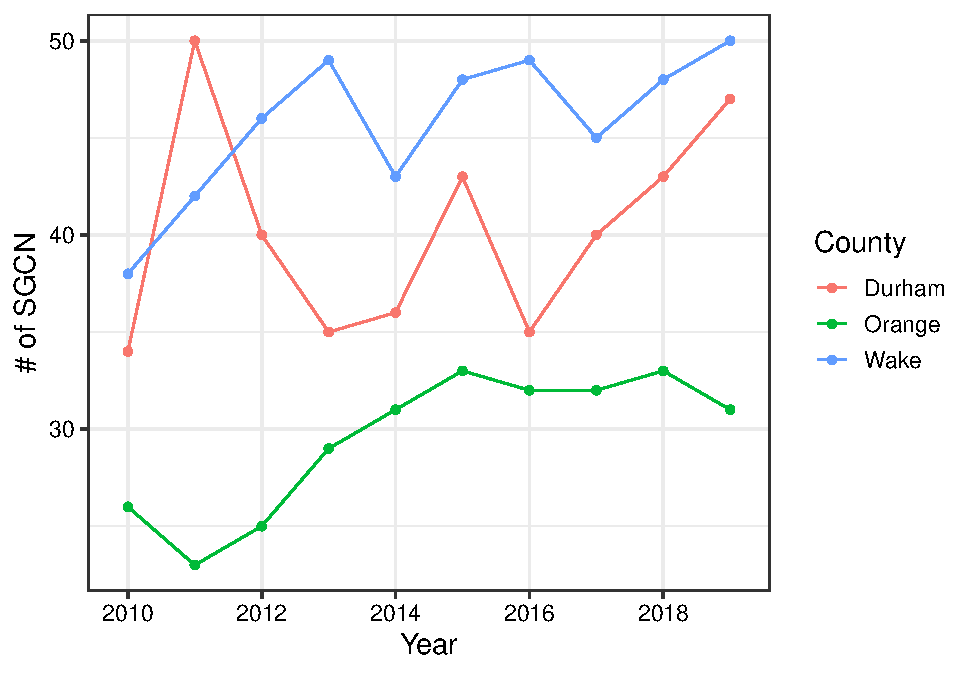
\includegraphics{Project_Template_files/figure-latex/SGCN code-1.pdf}

\begin{figure}
\centering
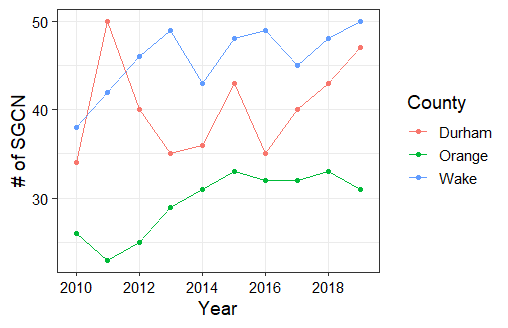
\includegraphics{./Output/SGCN_plot.png}
\caption{Figure 6. Number of SGCN observed in each county for each year
of the study period.}
\end{figure}

\hypertarget{question-2-how-did-the-popularity-of-ebird-change-in-the-research-triangle-across-the-2010s}{%
\subsection{Question 2: How did the popularity of eBird change in the
Research Triangle across the
2010s?}\label{question-2-how-did-the-popularity-of-ebird-change-in-the-research-triangle-across-the-2010s}}

A time series analysis of unique sampling events across all three
counties combined showed both a seasonal trend as well as a strong
positive monotonic trend (Figure 7). The seasonal trend in this time
series is likely related to a higher frequency in birding activity
during the spring migration and summer breeding season when weather
conditions are pleasant. Our visual assessment of the decomposition was
supported by a seasonal Mann-Kendall test that showed a significant
positive trend in species richness across the period (score = 520, tau =
0.963, p \textless{} 0.001). This trend was also consistent within each
county (Figures 8a-c). Additionally, seasonal Mann-Kendall tests showed
that this monotonic trend was significant for Durham (score = 283, tau =
0.525, p \textless{} 0.001), Orange (score = 495, tau = 0.918, p
\textless{} 0.001), and Wake counties (score = 514, tau = 0.952, p
\textless{} 0.001).

\begin{Shaded}
\begin{Highlighting}[]
\NormalTok{total.event.counts }\OtherTok{\textless{}{-}} \FunctionTok{read.csv}\NormalTok{(}\StringTok{"./Data/Processed/Total\_EventCounts.csv"}\NormalTok{)}
\NormalTok{total.event.counts }\OtherTok{\textless{}{-}}\NormalTok{ total.event.counts }\SpecialCharTok{\%\textgreater{}\%}
  \FunctionTok{group\_by}\NormalTok{(MY) }\SpecialCharTok{\%\textgreater{}\%}
  \FunctionTok{summarize}\NormalTok{(}\AttributeTok{total\_events =} \FunctionTok{sum}\NormalTok{(value))}

\CommentTok{\# Unique sampling events by month}
\NormalTok{Total.event.ts }\OtherTok{\textless{}{-}} \FunctionTok{ts}\NormalTok{(total.event.counts}\SpecialCharTok{$}\NormalTok{total\_events, }\AttributeTok{start =} \FunctionTok{c}\NormalTok{(}\DecValTok{2010}\NormalTok{,}\DecValTok{1}\NormalTok{), }\AttributeTok{frequency =} \DecValTok{12}\NormalTok{)}
\NormalTok{Total.event.decomp }\OtherTok{\textless{}{-}} \FunctionTok{stl}\NormalTok{(Total.event.ts, }\AttributeTok{s.window =} \StringTok{"periodic"}\NormalTok{)}
\FunctionTok{plot}\NormalTok{(Total.event.decomp)}
\end{Highlighting}
\end{Shaded}

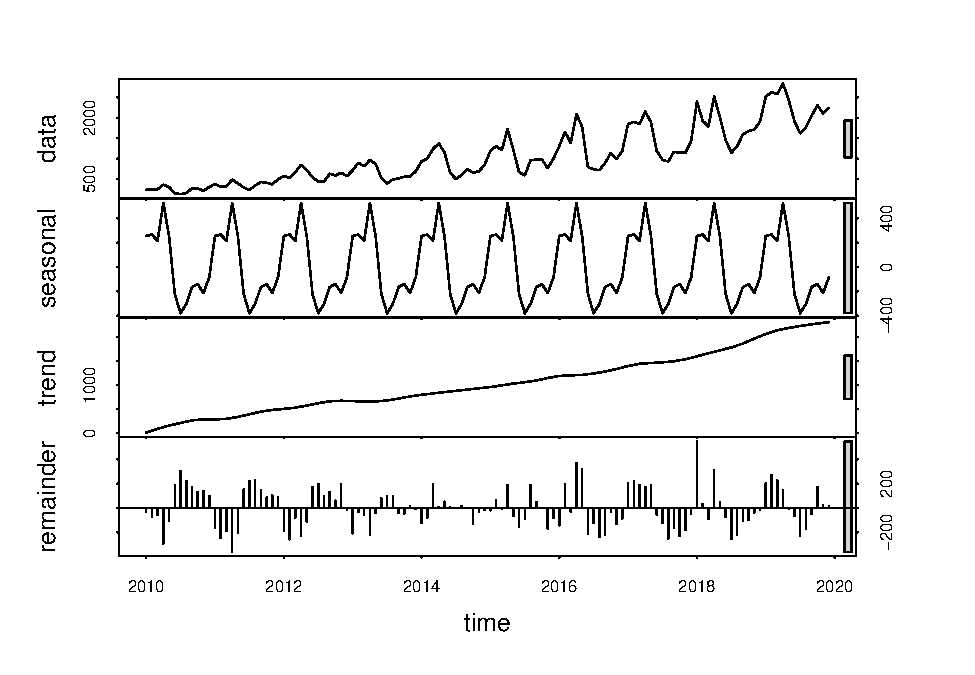
\includegraphics{Project_Template_files/figure-latex/Event TS Code-1.pdf}

\begin{Shaded}
\begin{Highlighting}[]
\NormalTok{Total.event.trend }\OtherTok{\textless{}{-}}\NormalTok{ Kendall}\SpecialCharTok{::}\FunctionTok{SeasonalMannKendall}\NormalTok{(Total.event.ts) }
\NormalTok{Total.event.trend}
\end{Highlighting}
\end{Shaded}

\begin{verbatim}
## tau = 0.963, 2-sided pvalue =< 2.22e-16
\end{verbatim}

\begin{Shaded}
\begin{Highlighting}[]
\FunctionTok{summary}\NormalTok{(Total.event.trend)}
\end{Highlighting}
\end{Shaded}

\begin{verbatim}
## Score =  520 , Var(Score) = 1500
## denominator =  540
## tau = 0.963, 2-sided pvalue =< 2.22e-16
\end{verbatim}

\begin{Shaded}
\begin{Highlighting}[]
\CommentTok{\# DURHAM}
\NormalTok{Durham.event.ts }\OtherTok{\textless{}{-}} \FunctionTok{ts}\NormalTok{(event.counts.Durham}\SpecialCharTok{$}\NormalTok{event\_total, }\AttributeTok{start =} \FunctionTok{c}\NormalTok{(}\DecValTok{2010}\NormalTok{,}\DecValTok{1}\NormalTok{), }\AttributeTok{frequency =} \DecValTok{12}\NormalTok{)}
\NormalTok{Durham.event.decomp }\OtherTok{\textless{}{-}} \FunctionTok{stl}\NormalTok{(Durham.event.ts, }\AttributeTok{s.window =} \StringTok{"periodic"}\NormalTok{)}
\FunctionTok{plot}\NormalTok{(Durham.event.decomp)}
\end{Highlighting}
\end{Shaded}

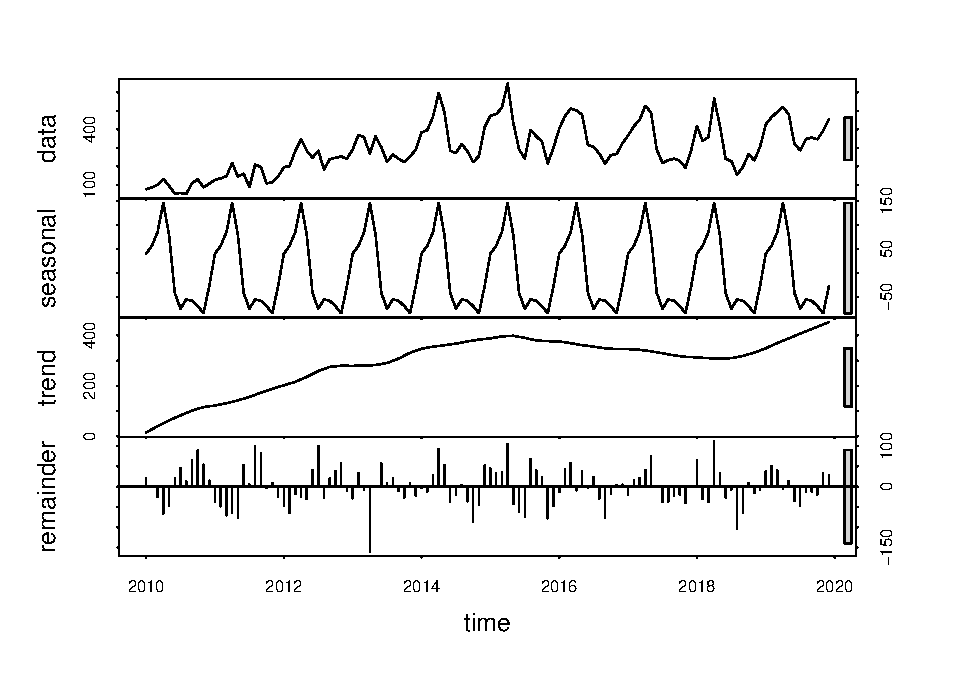
\includegraphics{Project_Template_files/figure-latex/Event TS Code-2.pdf}

\begin{Shaded}
\begin{Highlighting}[]
\NormalTok{Durham.event.trend }\OtherTok{\textless{}{-}}\NormalTok{ Kendall}\SpecialCharTok{::}\FunctionTok{SeasonalMannKendall}\NormalTok{(Durham.event.ts) }
\NormalTok{Durham.event.trend}
\end{Highlighting}
\end{Shaded}

\begin{verbatim}
## tau = 0.525, 2-sided pvalue =2.6823e-13
\end{verbatim}

\begin{Shaded}
\begin{Highlighting}[]
\FunctionTok{summary}\NormalTok{(Durham.event.trend)}
\end{Highlighting}
\end{Shaded}

\begin{verbatim}
## Score =  283 , Var(Score) = 1499
## denominator =  539.4972
## tau = 0.525, 2-sided pvalue =2.6823e-13
\end{verbatim}

\begin{Shaded}
\begin{Highlighting}[]
\CommentTok{\# ORANGE}
\NormalTok{Orange.event.ts }\OtherTok{\textless{}{-}} \FunctionTok{ts}\NormalTok{(event.counts.Orange}\SpecialCharTok{$}\NormalTok{event\_total, }\AttributeTok{start =} \FunctionTok{c}\NormalTok{(}\DecValTok{2010}\NormalTok{,}\DecValTok{1}\NormalTok{), }\AttributeTok{frequency =} \DecValTok{12}\NormalTok{)}
\NormalTok{Orange.event.decomp }\OtherTok{\textless{}{-}} \FunctionTok{stl}\NormalTok{(Orange.event.ts, }\AttributeTok{s.window =} \StringTok{"periodic"}\NormalTok{)}
\FunctionTok{plot}\NormalTok{(Orange.event.decomp)}
\end{Highlighting}
\end{Shaded}

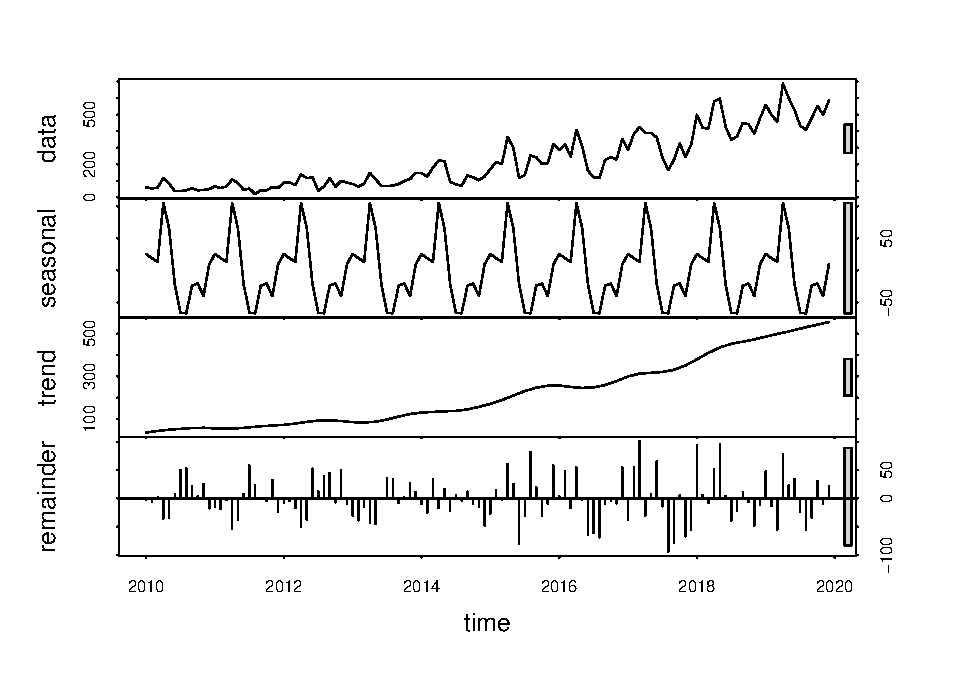
\includegraphics{Project_Template_files/figure-latex/Event TS Code-3.pdf}

\begin{Shaded}
\begin{Highlighting}[]
\NormalTok{Orange.event.trend }\OtherTok{\textless{}{-}}\NormalTok{ Kendall}\SpecialCharTok{::}\FunctionTok{SeasonalMannKendall}\NormalTok{(Orange.event.ts) }
\NormalTok{Orange.event.trend}
\end{Highlighting}
\end{Shaded}

\begin{verbatim}
## tau = 0.918, 2-sided pvalue =< 2.22e-16
\end{verbatim}

\begin{Shaded}
\begin{Highlighting}[]
\FunctionTok{summary}\NormalTok{(Orange.event.trend)}
\end{Highlighting}
\end{Shaded}

\begin{verbatim}
## Score =  495 , Var(Score) = 1499
## denominator =  539.4972
## tau = 0.918, 2-sided pvalue =< 2.22e-16
\end{verbatim}

\begin{Shaded}
\begin{Highlighting}[]
\CommentTok{\# WAKE}
\NormalTok{Wake.event.ts }\OtherTok{\textless{}{-}} \FunctionTok{ts}\NormalTok{(event.counts.Wake}\SpecialCharTok{$}\NormalTok{event\_total, }\AttributeTok{start =} \FunctionTok{c}\NormalTok{(}\DecValTok{2010}\NormalTok{,}\DecValTok{1}\NormalTok{), }\AttributeTok{frequency =} \DecValTok{12}\NormalTok{)}
\NormalTok{Wake.event.decomp }\OtherTok{\textless{}{-}} \FunctionTok{stl}\NormalTok{(Wake.event.ts, }\AttributeTok{s.window =} \StringTok{"periodic"}\NormalTok{)}
\FunctionTok{plot}\NormalTok{(Wake.event.decomp)}
\end{Highlighting}
\end{Shaded}

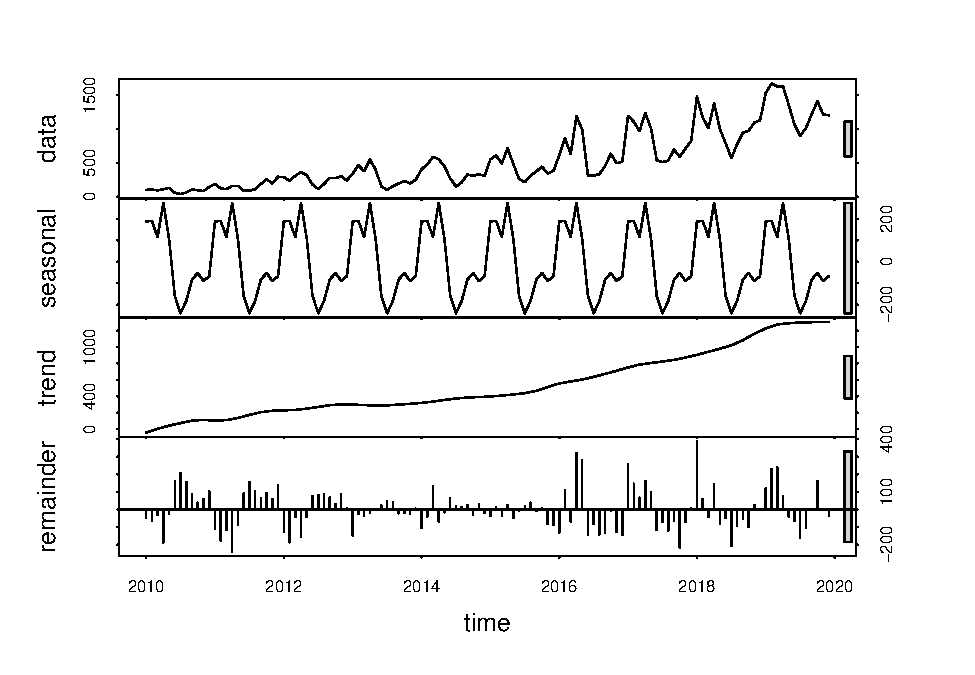
\includegraphics{Project_Template_files/figure-latex/Event TS Code-4.pdf}

\begin{Shaded}
\begin{Highlighting}[]
\NormalTok{Wake.event.trend }\OtherTok{\textless{}{-}}\NormalTok{ Kendall}\SpecialCharTok{::}\FunctionTok{SeasonalMannKendall}\NormalTok{(Wake.event.ts) }
\NormalTok{Wake.event.trend}
\end{Highlighting}
\end{Shaded}

\begin{verbatim}
## tau = 0.952, 2-sided pvalue =< 2.22e-16
\end{verbatim}

\begin{Shaded}
\begin{Highlighting}[]
\FunctionTok{summary}\NormalTok{(Wake.event.trend)}
\end{Highlighting}
\end{Shaded}

\begin{verbatim}
## Score =  514 , Var(Score) = 1500
## denominator =  540
## tau = 0.952, 2-sided pvalue =< 2.22e-16
\end{verbatim}

\begin{figure}
\centering
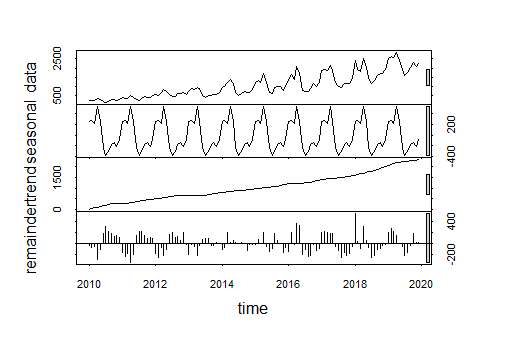
\includegraphics{./Output/RT_event_ts_decomp.png}
\caption{Figure 7. Time series decomposition for event count aggregated
across all three counties from 2010 to 2019.}
\end{figure}

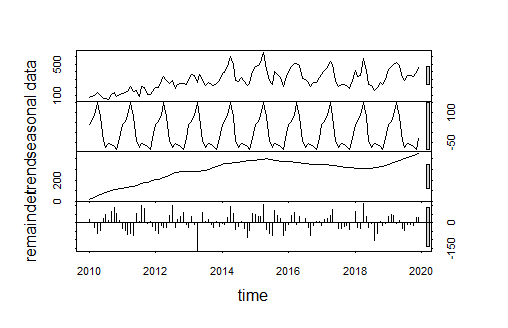
\includegraphics{./Output/Durham_event_ts_decomp.png}
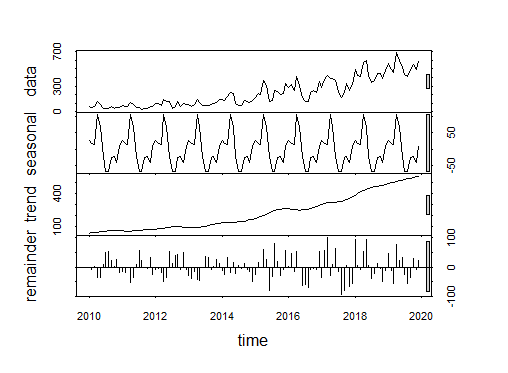
\includegraphics{./Output/Orange_event_ts_decomp.png}
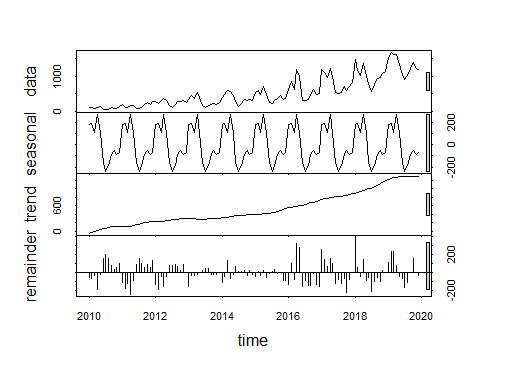
\includegraphics{./Output/Wake_event_ts_decomp.png}

In order to complete these time series analyses in R, we utilized the
zoo (Zeilies and Grothendeick 2005) and tseries (Trapletti and Hornik
2021) packages to construct the time series objects and the trend
(Pohlert 2020) and Kendall (McLeod 2011) packages to perform the
seasonal Mann-Kendall tests.

\newpage

\hypertarget{summary-and-conclusions}{%
\section{Summary and Conclusions}\label{summary-and-conclusions}}

According to our analysis of eBird data, species richness and diversity
increased in the Research Triangle between 2010 and 2019. This
conclusion does not support our initial hypothesis that diversity of the
Research Triangle's bird population would have decreased due to human
development. However, our other analyses invite the possibility that
this increase in species richness may be a product of confounding
variables.

Our time series analysis of unique sampling events across the decade
showed that eBird popularity drastically increased from 2010 to 2019. If
more people survey birds and upload their data, logically, this will
lead to more species being observed. Therefore, based on our analyses it
is not possible to say whether species richness increased, or how much
of this increase was caused by changes in eBird usage. The conclusion
that species richness increased is also not supported by the results of
our SGCN analysis, which did not show any clear trend over time. If
species diversity were increasing, it would be likely that the number of
SGCN observed in the Research Triangle was also increasing. Because of
this, we cannot make any definitive statements answering the question of
how bird diversity in the Research Triangle changed during the 2010s.

Despite our lack of conclusive results, researching changes in bird
populations across North America is incredibly important considering
past literature that has shown the risks they face. In terms of future
work related to this study, using a more consistent data source such as
the US Geological Survey Breeding Bird Survey (USGS BBS), which is
collected along pre-specified 25mi transects once a year, could help
illustrate the changes we were looking for without the confounding
variables brought on by the nature of open-source data. That being said,
citizen science and datahubs such as eBird are still very valuable for
conservation research and bolstering interest in environmental
protection among the wider public.

\newpage

\hypertarget{references}{%
\section{References}\label{references}}

Callaghan, CT, Major, RE, Wilshire, JH, Martin, JM, Kingsford, RT,
Cornwell, WK. 2019. Generalists are the most urban‐tolerant of birds: A
phylogenetically controlled analysis of ecological and life history
traits using a novel continuous measure of bird responses to
urbanization, Oikos. 128, 845-858.
\url{https://doi.org/10.1111/oik.06158}

Doran, EMB and Golden, JS. 2016. Climate \& Sustainability Implications
of Land Use Alterations in an Urbanizing Region: Raleigh-Durham, North
Carolina, Journal of Environmental Protection. 7, 1072-1088.
\url{http://dx.doi.org/10.4236/jep.2016.77096}

eBird Basic Dataset. Version: EBD\_relFeb-2022. Cornell Lab of
Ornithology, Ithaca, New York. Feb 2022.

McLeod, AI. 2011. Kendall: Kendall rank correlation and Mann-Kendall
trend test. R package version 2.2.
\url{https://CRAN.R-project.org/package=Kendall}

Minor, E, Urban, D. 2010. Forest bird communities across a gradient of
urban development, Urban Ecosystems. 13, 51-71.
\url{https://doi.org/10.1007/s11252-009-0103-1}

North Carolina Wildlife Resources Commission. 2020. Addendum 1 to the
Wildlife Action Plan. Raleigh, NC. \url{https://www.ncwildlife.org/plan}

Pohlert, T. 2020. trend: Non-Parametric Trend Tests and Change-Point
Detection. R package version 1.1.4.
\url{https://CRAN.R-project.org/package=trend}

R Core Team. 2021. R: A language and environment for statistical
computing. R Foundation for Statistical Computing, Vienna, Austria.
\url{https://www.R-project.org/}

Rosenberg, KV, Dokter, AM, Blancher, PJ, Sauer JR, Smith, AC, Smith, PA,
Stanton, JC, Panjabi, A, Helft, L, Parr, M, and Marra, PP. 2019. Decline
of the North American avifauna, Science. 366, 120-124.
\url{https://doi.org/10.1126/science.aaw1313}

Şekercioğlu, ÇH, Daily, GC, Ehrlich, PR. 2004. Ecosystem consequences of
bird declines, Proceedings of the National Academy of Sciences of the
United States of America. 101, 18042-18047.
\url{https://doi.org/10.1073/pnas.0408049101}

Trapletti, A and Hornik, K. 2021. tseries: Time Series Analysis and
Computational Finance. R package version 0.10-49.

Wickham, H, Averick, M, Bryan, J, Chang, W, D'Agostino McGowan, L,
François, R, Grolemund, G, Hayes, A, Henry, L, Hester, J, Kuhn, M ,
Pedersen, TL, Miller, E, Bache, SM, Müller, K, Ooms, J, Robinson, D,
Seidel, DP, Spinu, V, Takahashi, K, Vaughan, D, Wilke, C,Woo, K, and
Hiroaki Yutani, H. 2019. Welcome to the tidyverse. Journal of Open
Source Software. 4, 1686. \url{https://doi.org/10.21105/joss.01686}

Zeileis, A and Grothendieck, G. 2005. zoo: S3 Infrastructure for Regular
and Irregular Time Series. Journal of Statistical Software. 14, 1-27.
\url{doi:10.18637/jss.v014.i06}

\end{document}
